\documentclass[10pt]{article}

\usepackage[a4paper,margin=20mm]{geometry}
\usepackage{amsmath}
\usepackage{booktabs}
\usepackage{graphicx}
\usepackage{xcolor}
\usepackage{caption}

\captionsetup{font=small}
\newcommand{\revisionpending}{\textcolor{red}{\textbf{GPU result pending}}}

\begin{document}

\setcounter{figure}{0}
\renewcommand{\thefigure}{S\arabic{figure}}
\setcounter{table}{0}
\renewcommand{\thetable}{S\arabic{table}}

\begin{center}
{\Large\bfseries Supplementary material}\par
\medskip
{\large Angle-domain null subtraction imaging from beamformed plane-wave data}\par
\medskip
Henri Leroy
\end{center}

\section*{S1. Paired-angle null and small-angle approximation}

For a symmetric set of steering angles and equal complex pair amplitudes, the
exact antisymmetric pair response is
\begin{equation}
B_{+\theta}-B_{-\theta}=-2\mathrm{i}A_\theta
\sin(k_0\Delta x\sin\theta),
\end{equation}
which becomes $-2\mathrm{i}A_\theta k_0\Delta x\sin\theta$ near the
focus. Figure~\ref{fig:s1} verifies the local approximation and shows the
normalized null slope as angle count and total span change. Raw sign weights
sum to zero for paired angles under nonuniform sampling; broadside has zero
null weight. Unpaired sequences require a separately designed null because
response symmetry depends on physically paired acquisitions.

Using the NSI functional from the manuscript, and writing $S=\sum_{\theta>0}A_\theta\sin\theta$, this gives:
\begin{equation}
E_\theta(\Delta x)\simeq
\frac{\left|cU(\Delta x)-2\mathrm{i}k_0\Delta x S\right|
+\left|cU(\Delta x)+2\mathrm{i}k_0\Delta x S\right|}{2}
-2k_0|\Delta x|\,|S|
\label{eq:angle-local-psf-expanded}
\end{equation}

The subtraction also depends on the relative amplitude and phase of \(Z\) and \(U\). For $c|U|>0$, define $\rho=|Z|/(c|U|)$ and, when $Z\ne0$, $\psi=\arg Z-\arg U$.
The normalized response is:
\begin{equation}
    \frac{\mathcal{N}(U,Z;c)}{c|U|}
=\frac{|1+\rho e^{\mathrm{i}\psi}|+|1-\rho e^{\mathrm{i}\psi}|}{2}-\rho
\end{equation}

At $Z=0$, the normalized response equals one.

\begin{figure}[h]
\centering
\IfFileExists{supplementary/figureS1_angular_null_theory.png}{%
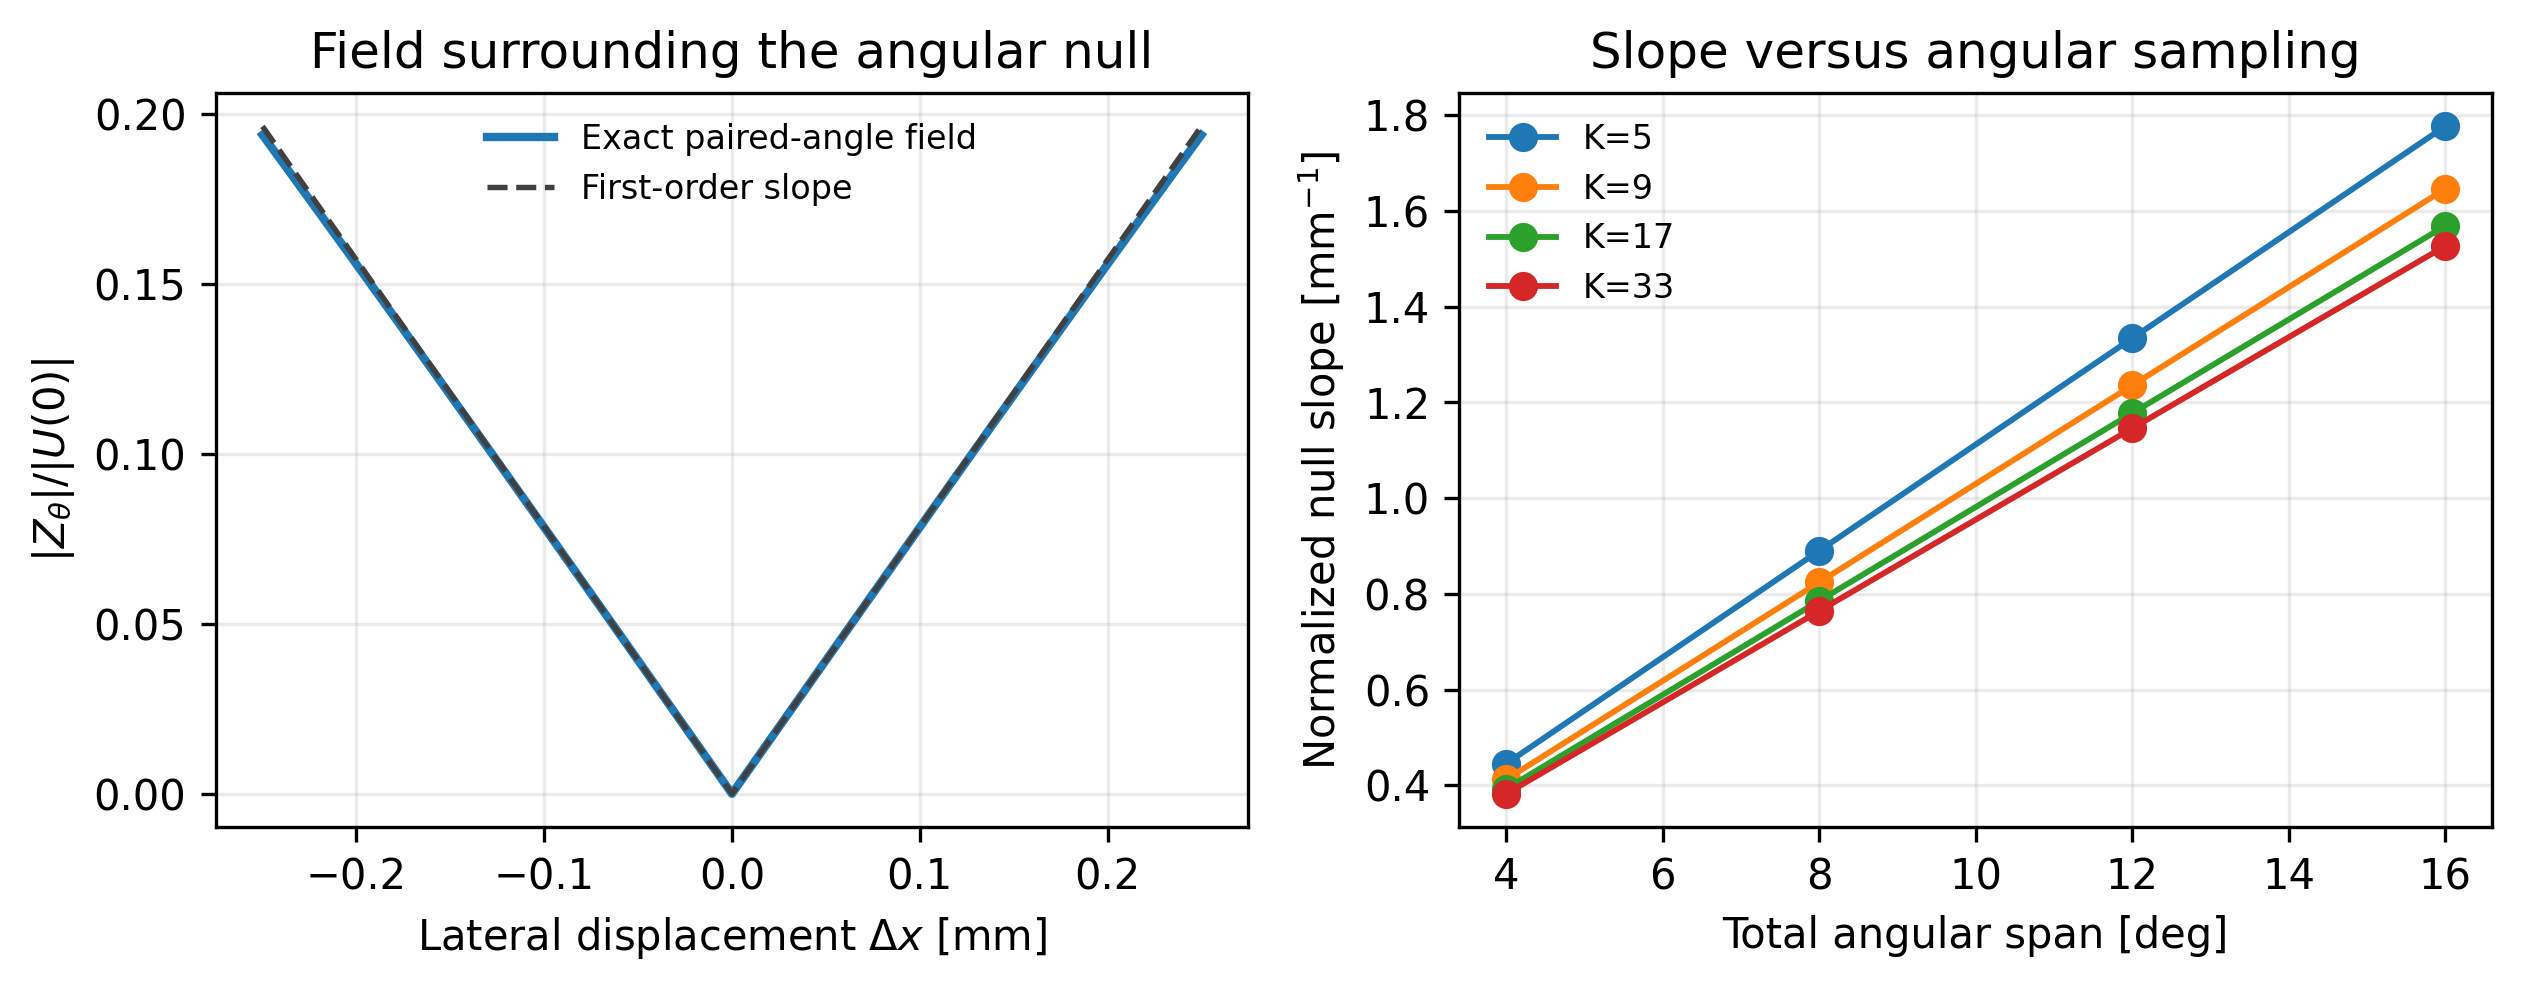
\includegraphics[width=0.94\textwidth]{supplementary/figureS1_angular_null_theory.png}}{%
\fbox{\parbox{0.85\textwidth}{\centering\revisionpending:\ angular-null figure}}}
\caption{Physical interpretation of the angular null. The exact symmetric-pair
field is compared with its first-order small-angle approximation, and the
normalized slope is shown versus angular span and sampling.}
\label{fig:s1}
\end{figure}

\clearpage
\section*{S2. Angular sampling and missing-transmission tests}

The angle-count sweep retained an 8$^\circ$ total span, and the span sweep
retained 17 uniformly spaced transmissions. The missing-angle experiment
removed the $+2^\circ$ acquisition. ``Raw sign'' retained
$v_k=\operatorname{sign}(\theta_k)$, leaving a weight sum of $-1$;
``recentered'' subtracted the mean of the remaining weights. The recentered
case differed from the symmetric baseline: Angle-NSI width increased from
0.116 to 0.193 mm and the peak shifted by 0.059 mm.

\begin{figure}[h]
\centering
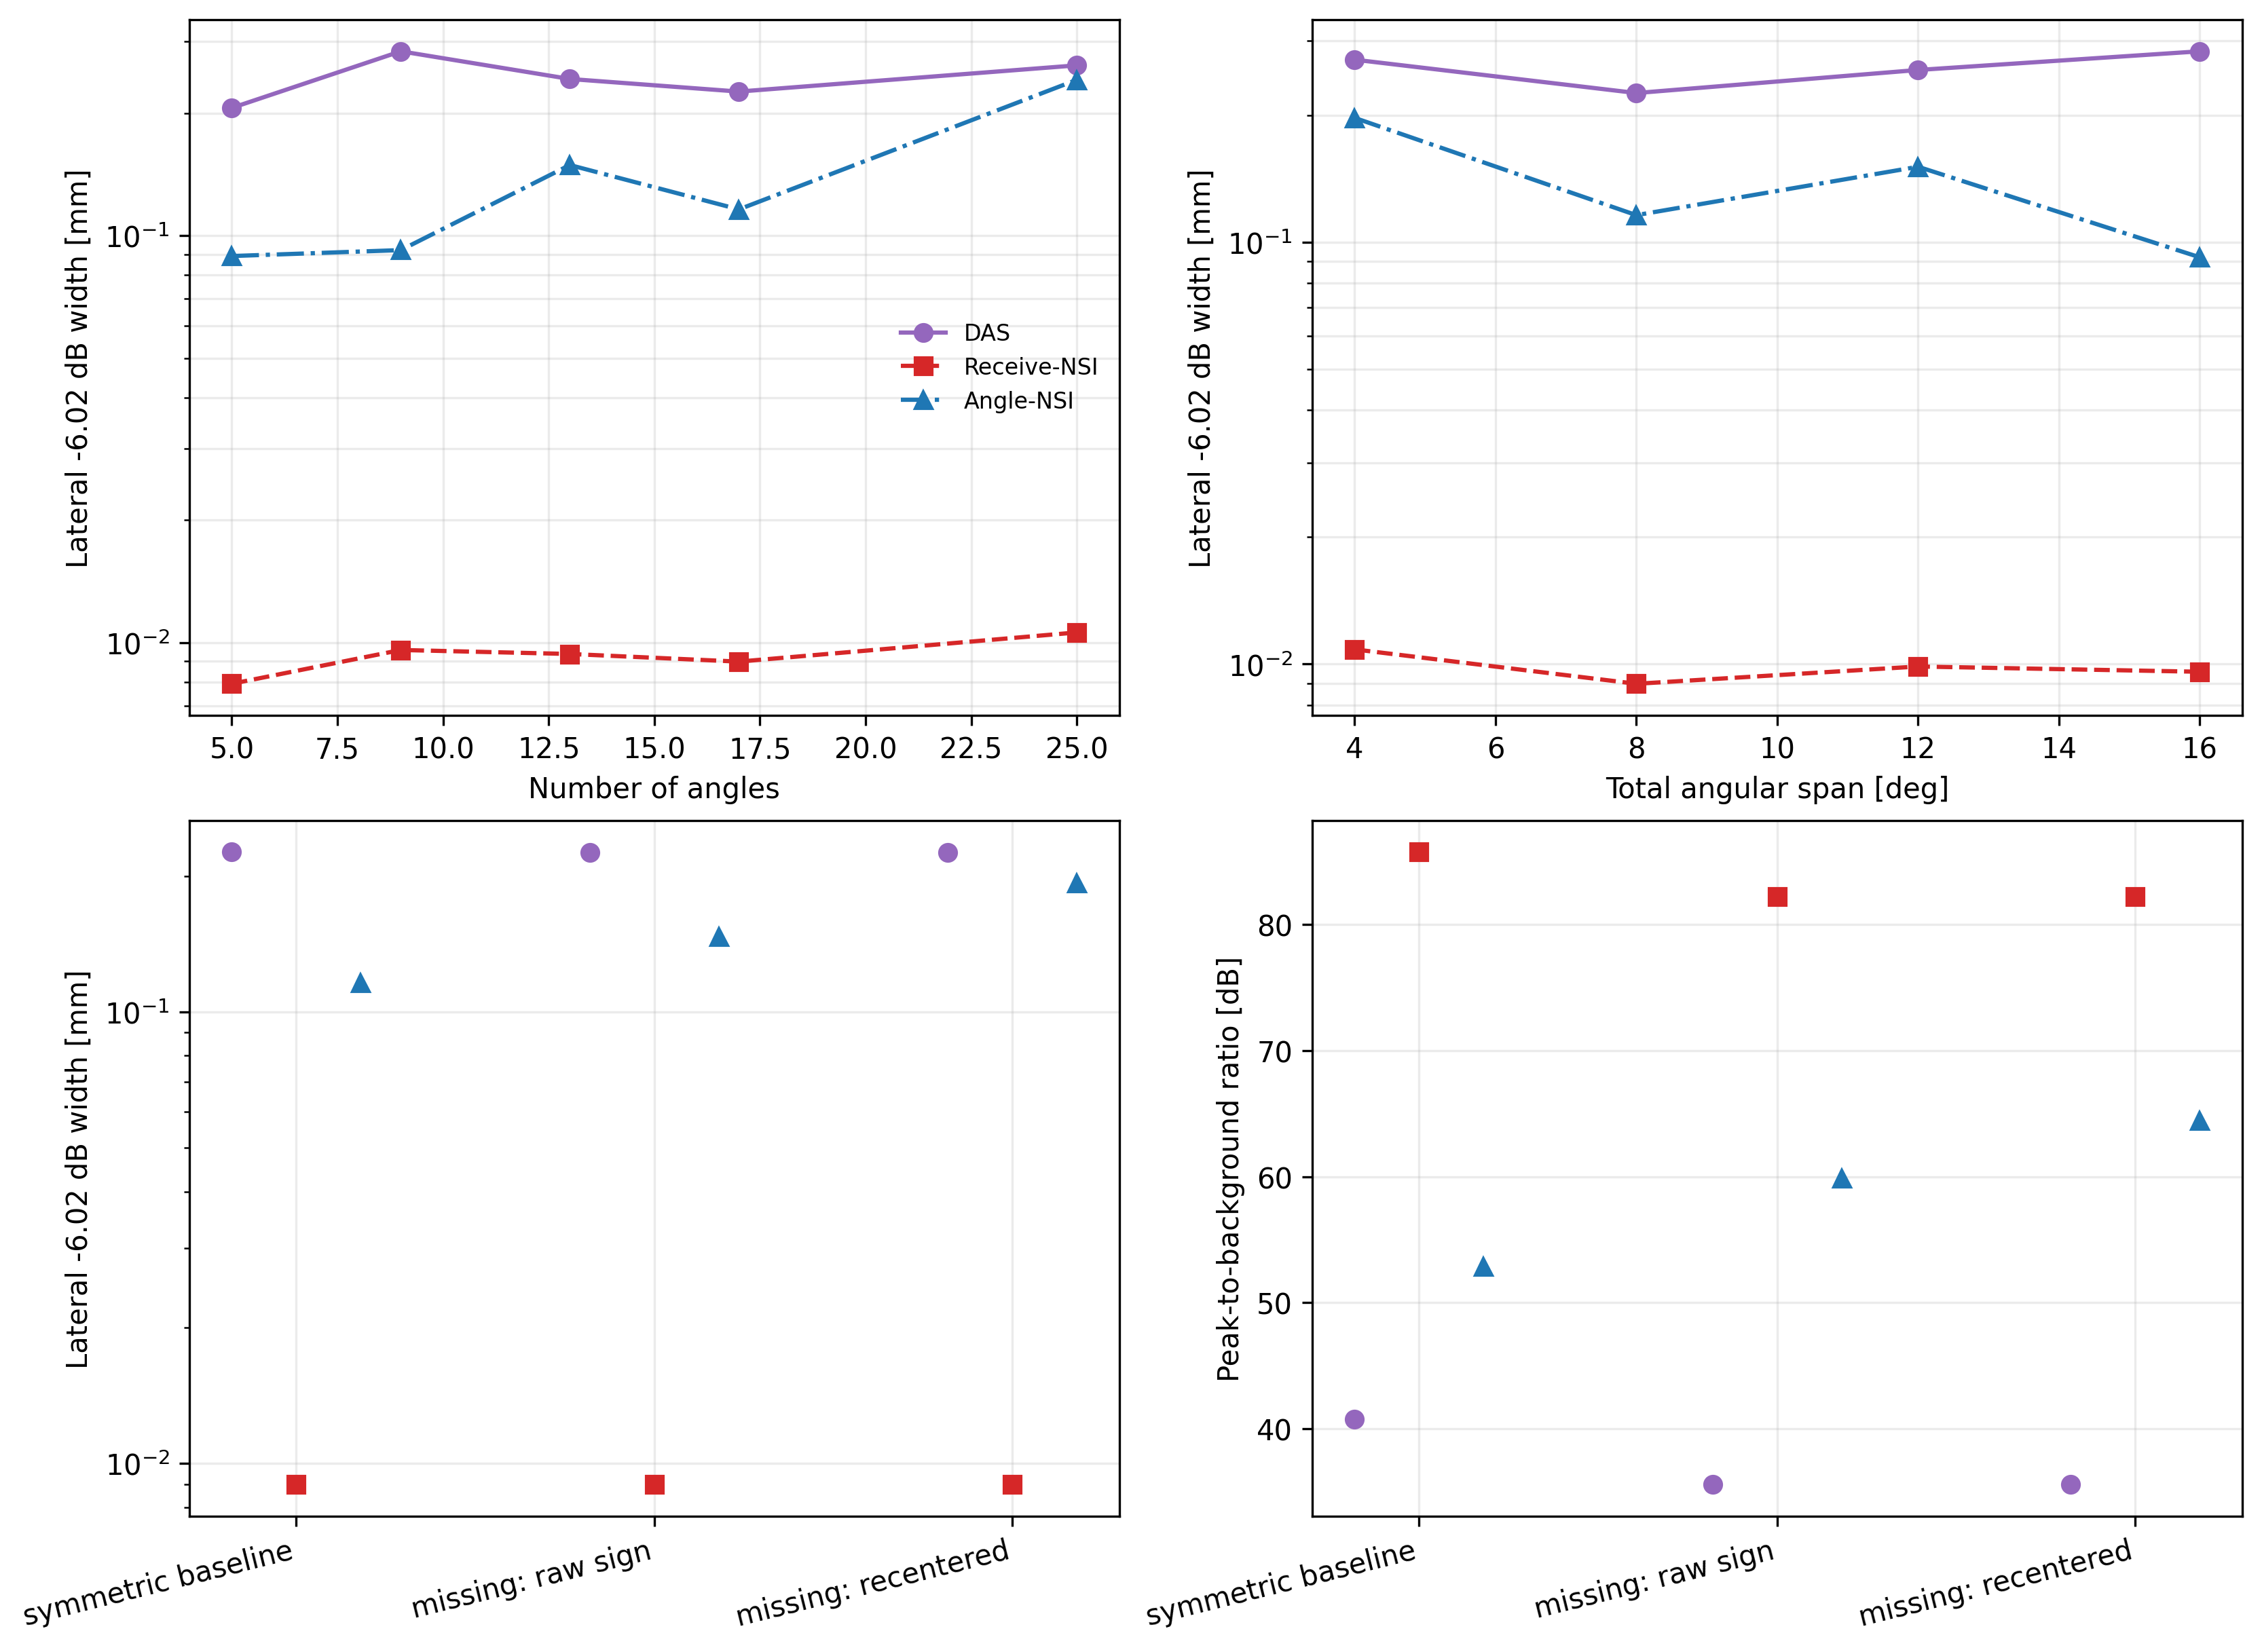
\includegraphics[width=0.90\textwidth]{supplementary/figureS1_angle_sweeps.png}
\caption{Robustness to angular sampling. Top: lateral $-6$ dB width versus
angle count and total angular span. Bottom: width and peak-to-background level
for the symmetric baseline and two missing-angle weight strategies.}
\label{fig:s2}
\end{figure}

\clearpage
\section*{S3. Additive-noise and phase-jitter tests}

Noise SNR is the global complex-IQ root-mean-square amplitude divided by the
root-mean-square amplitude of additive complex noise. Phase jitter is an
independent Gaussian phase offset applied to each complete per-angle IQ
acquisition. Values below are mean $\pm$ sample standard deviation over ten
realizations. The noiseless and zero-jitter baselines are deterministic.

\begin{table}[h]
\centering
\caption{Selected Angle-NSI lateral $-6$ dB widths.}
\begin{tabular}{@{}lcc@{}}
\toprule
Perturbation & Level & Width (mm) \\
\midrule
None & -- & 0.11595 \\
Complex-IQ noise & 40 dB & $0.11620\pm0.00019$ \\
 & 20 dB & $0.11722\pm0.00203$ \\
 & 10 dB & $0.12197\pm0.00487$ \\
Inter-angle phase jitter & 2$^\circ$ & $0.14374\pm0.02581$ \\
 & 5$^\circ$ & $0.16669\pm0.02301$ \\
 & 10$^\circ$ & $0.19385\pm0.02906$ \\
 & 20$^\circ$ & $0.18316\pm0.05501$ \\
\bottomrule
\end{tabular}
\end{table}

\begin{figure}[h]
\centering
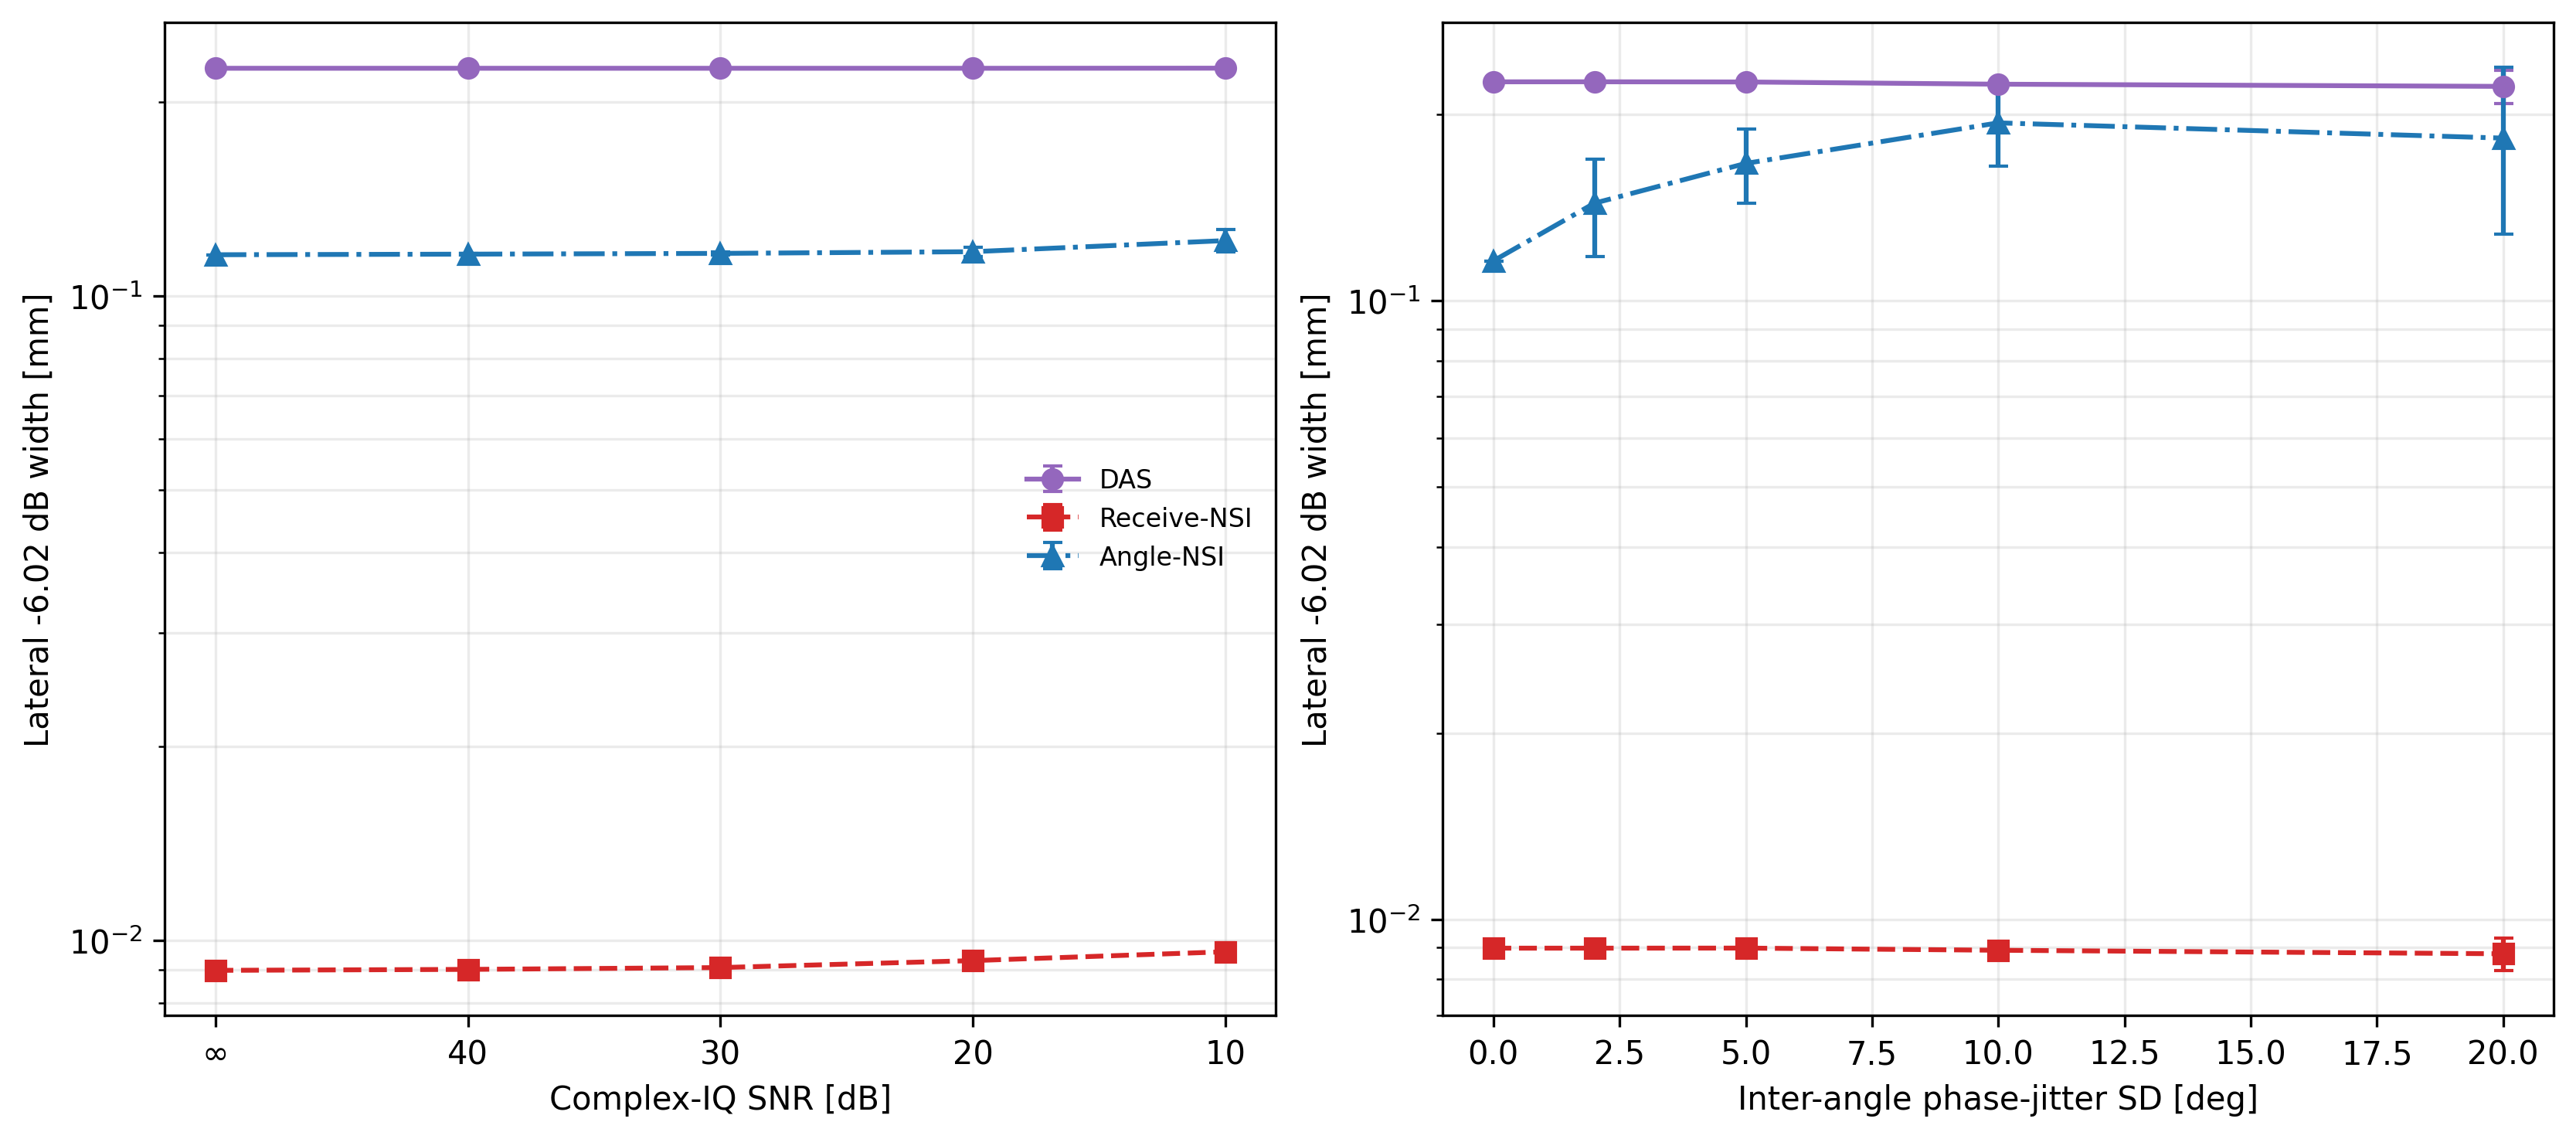
\includegraphics[width=0.93\textwidth]{supplementary/figureS2_noise_phase_sweeps.png}
\caption{Mean Angle-NSI lateral $-6$ dB width under additive complex-IQ noise
(left) and inter-angle phase jitter (right). Error bars are sample standard
deviations over ten realizations.}
\label{fig:s3}
\end{figure}

\clearpage
\section*{S4. Simulated spatial point-target response}

Each depth was tested at $x=-4$, 0 and 4 mm. Angle-NSI was laterally consistent
at a given depth (largest sample standard deviation 0.00172 mm). Receive-NSI
had a narrow centered response and wider, shifted off-axis responses, producing
the larger within-depth dispersions in table~\ref{tab:s4}.

\begin{table}[h]
\centering
\caption{Mean $\pm$ sample standard deviation of lateral width over three
lateral positions.}
\label{tab:s4}
\begin{tabular}{@{}rccc@{}}
\toprule
Depth (mm) & DAS (mm) & Receive-NSI (mm) & Angle-NSI (mm) \\
\midrule
15 & $0.1972\pm0.0007$ & $0.0514\pm0.0380$ & $0.0636\pm0.0017$ \\
20 & $0.2275\pm0.0015$ & $0.0565\pm0.0412$ & $0.1177\pm0.0015$ \\
25 & $0.2315\pm0.0033$ & $0.0530\pm0.0381$ & $0.1181\pm0.0014$ \\
30 & $0.2405\pm0.0036$ & $0.0478\pm0.0333$ & $0.1144\pm0.0015$ \\
\bottomrule
\end{tabular}
\end{table}

\begin{figure}[h]
\centering
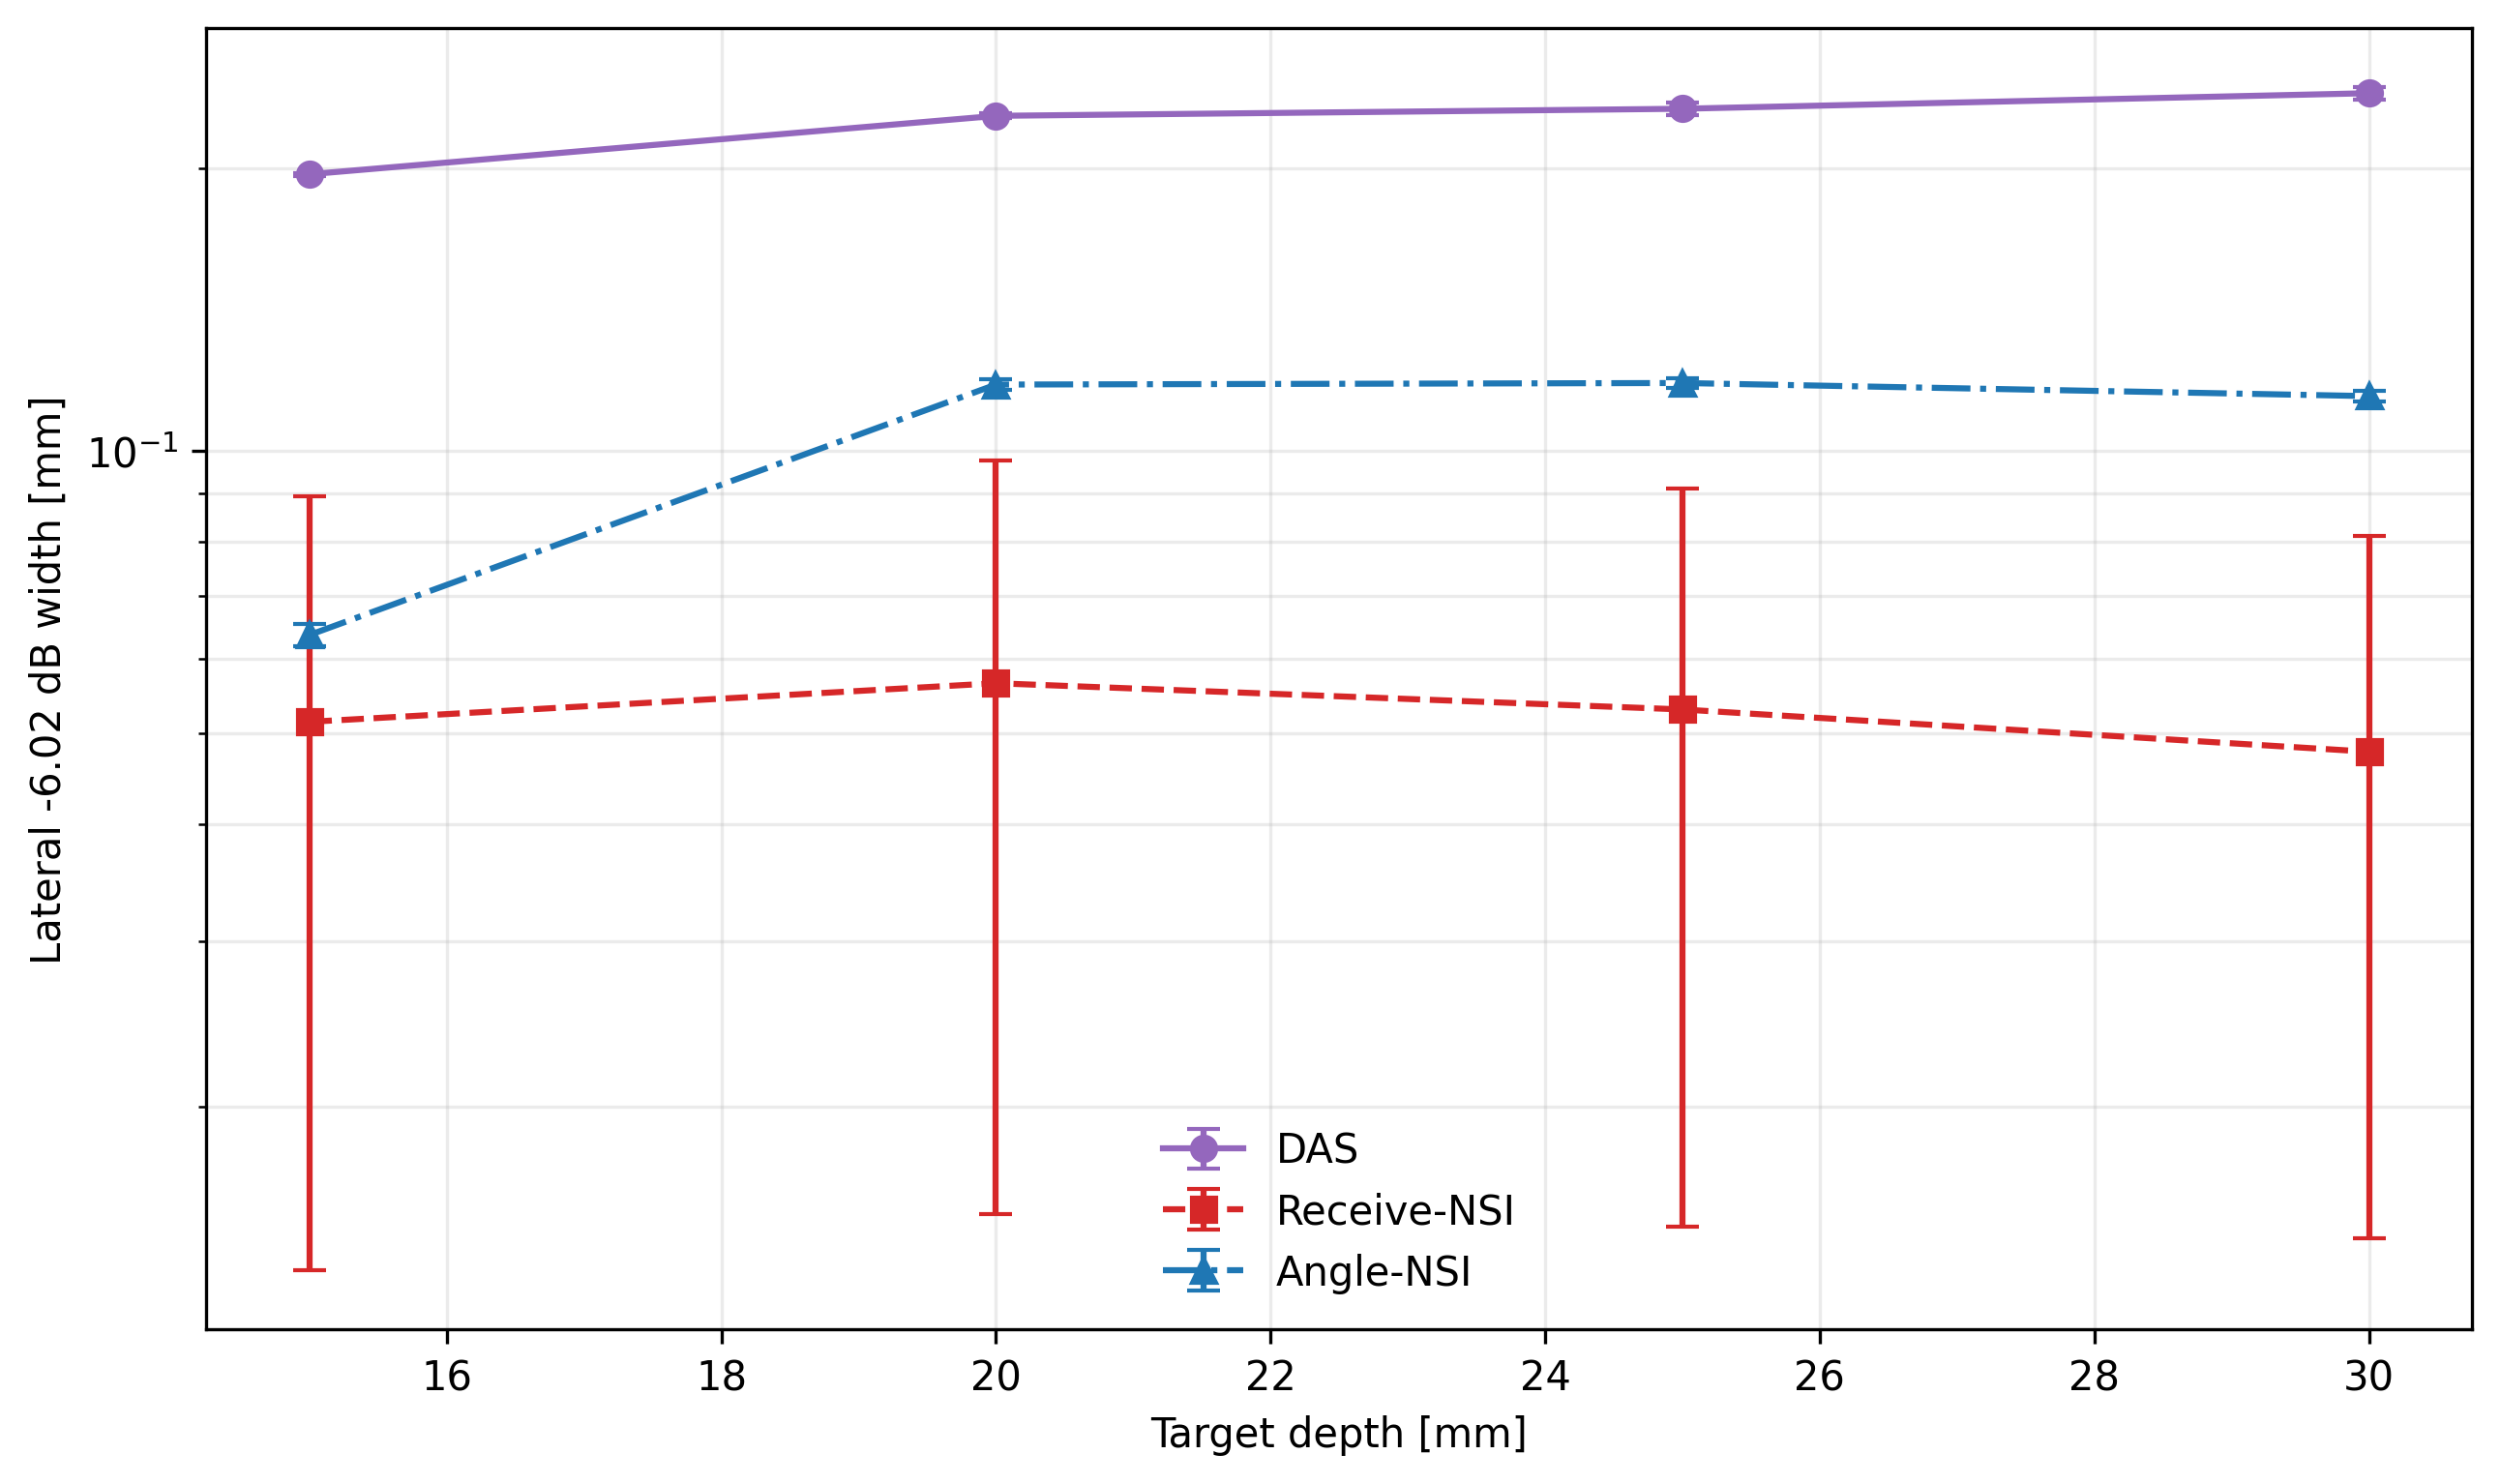
\includegraphics[width=0.80\textwidth]{supplementary/figureS3_spatial_psf.png}
\caption{Lateral $-6$ dB width versus target depth, summarized over three
lateral positions. Points are means and error bars are sample standard
deviations.}
\label{fig:s4}
\end{figure}

\begin{table}[h]
\centering
\caption{Six-method simulated point-target metrics. Widths are measured on
uncompressed envelopes at $-6$ dB. Map-slice spacing is 0.02 mm;
Receive-NSI uses the validated 0.000390625 mm fine grid.}
\label{tab:s4-six-method}
\resizebox{\textwidth}{!}{\begin{tabular}{@{}lrrrr@{}}
\toprule
Method & Lateral width (mm) & Axial width (mm) & Peak/background (dB) & Centre/peak (dB) \\
\midrule
DAS & 0.2255 & 0.7202 & 56.9 & 0.0 \\
CF-DAS & 0.1459 & 0.4835 & 90.6 & 0.0 \\
MV & 0.1743 & 0.7342 & 73.5 & 0.0 \\
DMAS & 0.3706 & 0.1383 & 63.4 & $-0.2$ \\
Receive-NSI & 0.0090 & 0.7202 & 120.4 & 0.0 \\
Angle-NSI & 0.1160 & 0.7202 & 95.9 & 0.0 \\
\bottomrule
\end{tabular}
}
\end{table}

\clearpage
\section*{S5. Simulated point-target sensitivity to the NSI offset}

The same complex reference and null fields were reused at $c=0.02$, 0.05, 0.10
and 0.20. Width and peak-to-profile-background level are reported together
because $c$ changes both the sharpness and retained output.

\begin{figure}[h]
\centering
\IfFileExists{supplementary/figureS5_point_target_c_sensitivity.png}{%
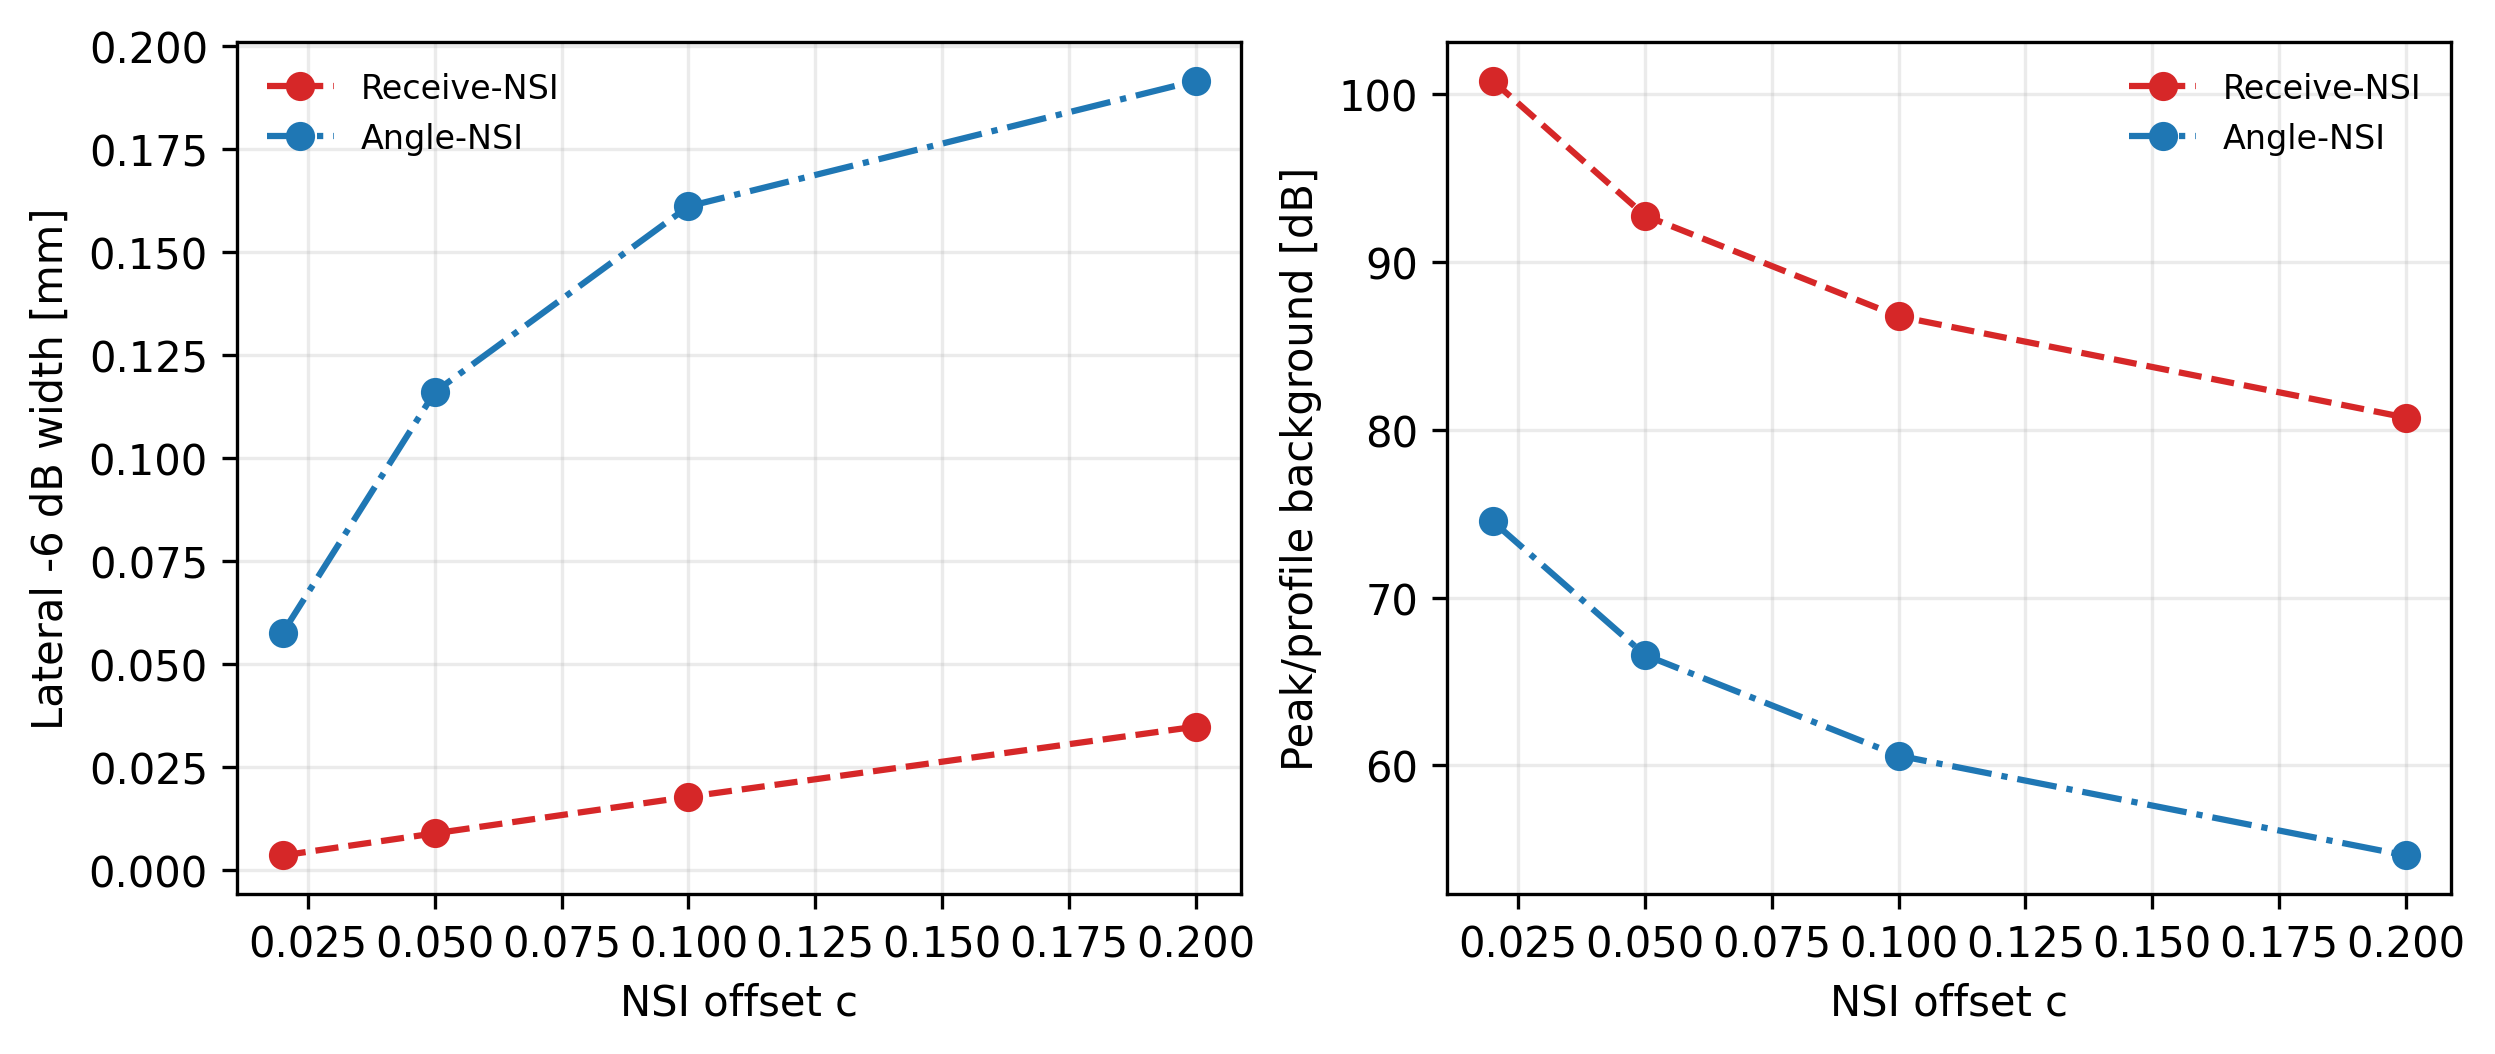
\includegraphics[width=0.90\textwidth]{supplementary/figureS5_point_target_c_sensitivity.png}}{%
\fbox{\parbox{0.85\textwidth}{\centering\revisionpending:\ simulated $c$-sensitivity figure}}}
\caption{Receive-NSI and Angle-NSI lateral $-6$ dB width and
peak-to-profile-background level versus $c$.}
\label{fig:s5}
\end{figure}

\clearpage
\section*{S6. MBTrace positional concordance}

DAS is a reconstruction reference, not independent microbubble ground truth.
The tolerance curves in figure~\ref{fig:s6} therefore quantify positional
concordance. The displacement audit in table~\ref{tab:s6} first locks
assignments within 0.15 mm and then assigns residual peaks within the 0.35 mm
tracking radius.

\begin{figure}[h]
\centering
\IfFileExists{supplementary/figureS6_mbtrace_concordance.png}{%
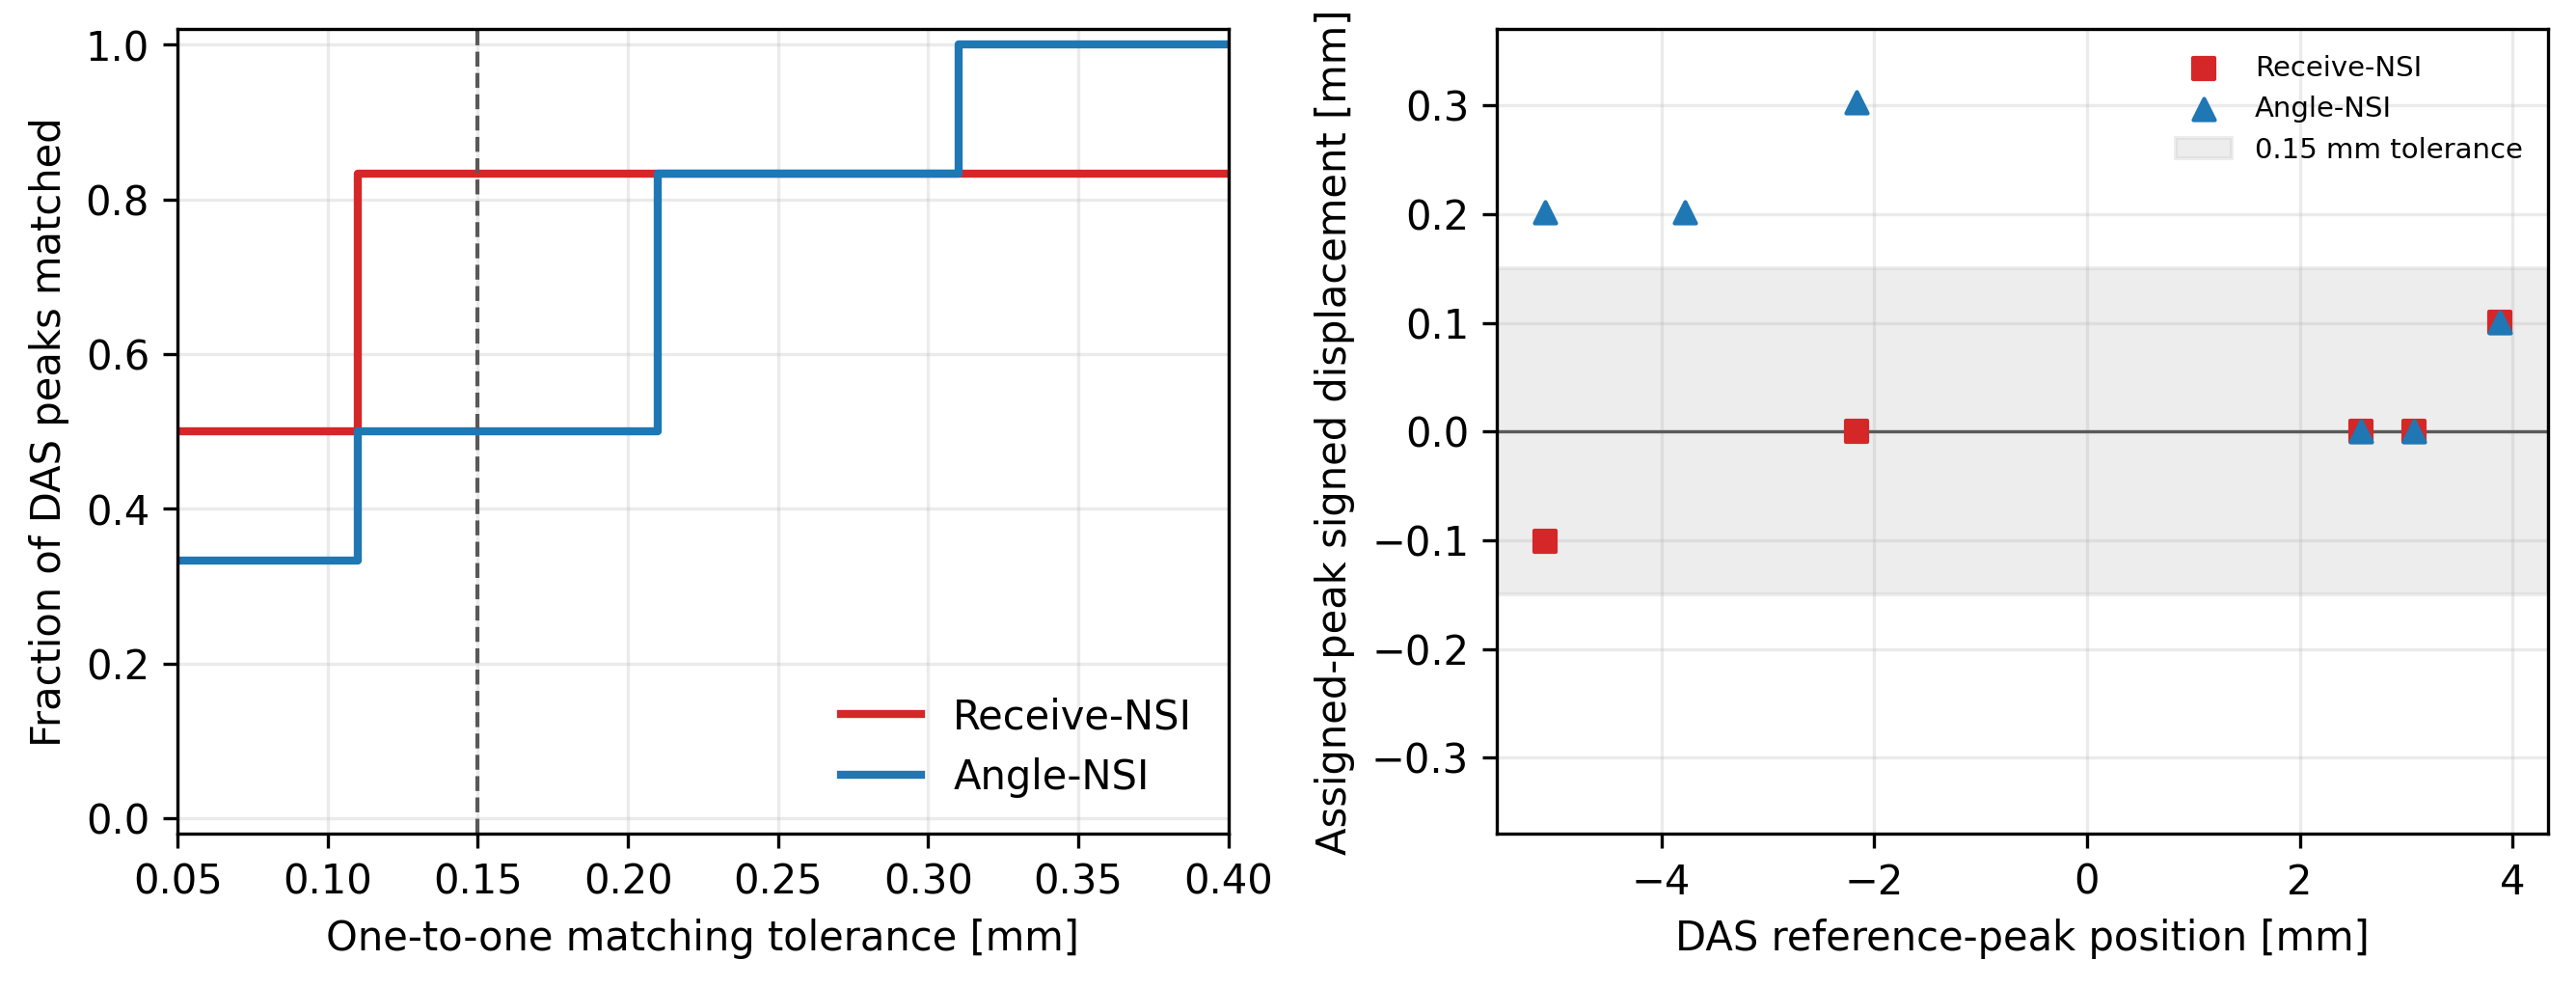
\includegraphics[width=0.92\textwidth]{supplementary/figureS6_mbtrace_concordance.png}}{%
\fbox{\parbox{0.85\textwidth}{\centering\revisionpending:\ MBTrace concordance figure}}}
\caption{Fraction of six DAS peaks assigned versus tolerance (left) and signed
displacement under the two-stage audit (right).}
\label{fig:s6}
\end{figure}

\begin{table}[h]
\centering
\caption{MBTrace one-to-one displacement audit. ``No peak'' means that no
unassigned target peak lay within the 0.35 mm tracking radius.}
\label{tab:s6}
\resizebox{\textwidth}{!}{\begin{tabular}{@{}lrrrrl@{}}
\toprule
Method & DAS peak & Assigned peak & Signed shift & Absolute shift & Classification \\
\midrule
Receive-NSI & -5.092 & -5.193 & -0.101 & 0.101 & matched within tolerance \\
Receive-NSI & -3.782 & -- & -- & -- & no peak within tracking radius \\
Receive-NSI & -2.168 & -2.168 & 0.000 & 0.000 & matched within tolerance \\
Receive-NSI & 2.571 & 2.571 & 0.000 & 0.000 & matched within tolerance \\
Receive-NSI & 3.076 & 3.076 & 0.000 & 0.000 & matched within tolerance \\
Receive-NSI & 3.882 & 3.983 & 0.101 & 0.101 & matched within tolerance \\
Angle-NSI & -5.092 & -4.891 & 0.202 & 0.202 & displaced beyond matching tolerance \\
Angle-NSI & -3.782 & -3.580 & 0.202 & 0.202 & displaced beyond matching tolerance \\
Angle-NSI & -2.168 & -1.866 & 0.303 & 0.303 & displaced beyond matching tolerance \\
Angle-NSI & 2.571 & 2.571 & 0.000 & 0.000 & matched within tolerance; possible split \\
Angle-NSI & 3.076 & 3.076 & 0.000 & 0.000 & matched within tolerance \\
Angle-NSI & 3.882 & 3.983 & 0.101 & 0.101 & matched within tolerance \\
\bottomrule
\end{tabular}
}
\end{table}

\clearpage
\section*{S7. MBTrace sensitivity to the NSI offset}

The primary $c=0.10$ reproduces the $d_c=0.10$ value used by Kou
\textit{et al.} and the corresponding released Open-NSI configuration; it was
fixed before the present MBTrace analysis. The strict and wider matching
fractions, detected counts, width and amplitude diagnostics were recomputed at
all four values.

\begin{figure}[h]
\centering
\IfFileExists{supplementary/figureS7_mbtrace_c_sensitivity.png}{%
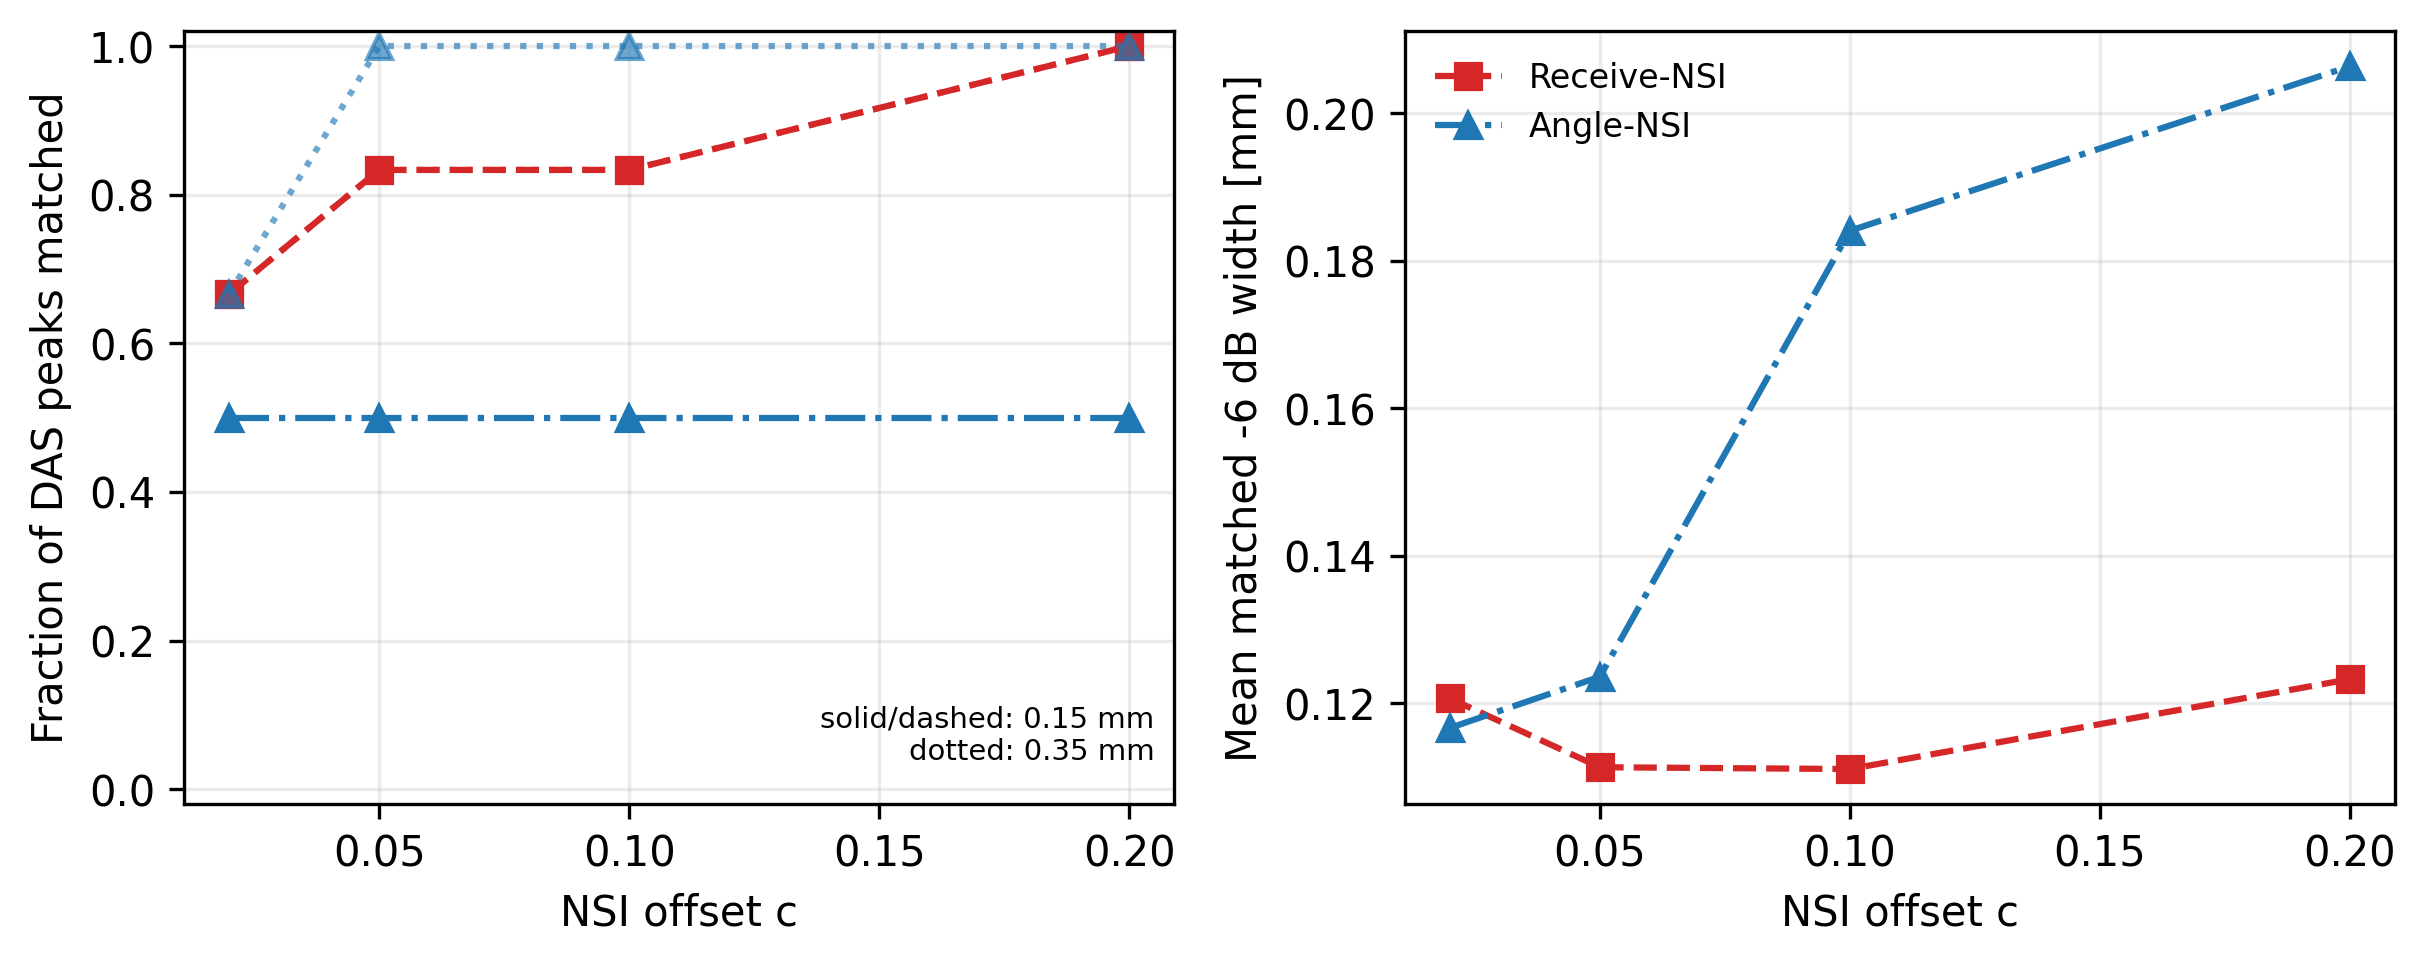
\includegraphics[width=0.90\textwidth]{supplementary/figureS7_mbtrace_c_sensitivity.png}}{%
\fbox{\parbox{0.85\textwidth}{\centering\revisionpending:\ MBTrace $c$-sensitivity figure}}}
\caption{MBTrace positional concordance at 0.15 and 0.35 mm tolerances and
mean strictly matched width versus $c$.}
\label{fig:s7}
\end{figure}

\begin{table}[h]
\centering
\caption{MBTrace peak counts and DAS concordance versus $c$.}
\label{tab:s7}
\resizebox{\textwidth}{!}{\begin{tabular}{@{}lrrrr@{}}
\toprule
Method & $c$ & Detected peaks & Match at 0.15 mm & Match at 0.35 mm \\
\midrule
Receive-NSI & 0.02 & 5 & 66.7\% & 66.7\% \\
Angle-NSI & 0.02 & 4 & 50.0\% & 66.7\% \\
Receive-NSI & 0.05 & 6 & 83.3\% & 83.3\% \\
Angle-NSI & 0.05 & 7 & 50.0\% & 100.0\% \\
Receive-NSI & 0.10 & 6 & 83.3\% & 83.3\% \\
Angle-NSI & 0.10 & 7 & 50.0\% & 100.0\% \\
Receive-NSI & 0.20 & 8 & 100.0\% & 100.0\% \\
Angle-NSI & 0.20 & 8 & 50.0\% & 100.0\% \\
\bottomrule
\end{tabular}
}
\end{table}

\clearpage
\section*{S8. Carotid sensitivity to the NSI offset}

The fixed lumen and tissue masks from the primary analysis were retained at all
$c$ values. Every image is derived from the same complex reference and null
fields, so this sweep isolates the subtraction offset.

\begin{figure}[h]
\centering
\IfFileExists{supplementary/figureS8_carotid_c_sensitivity.png}{%
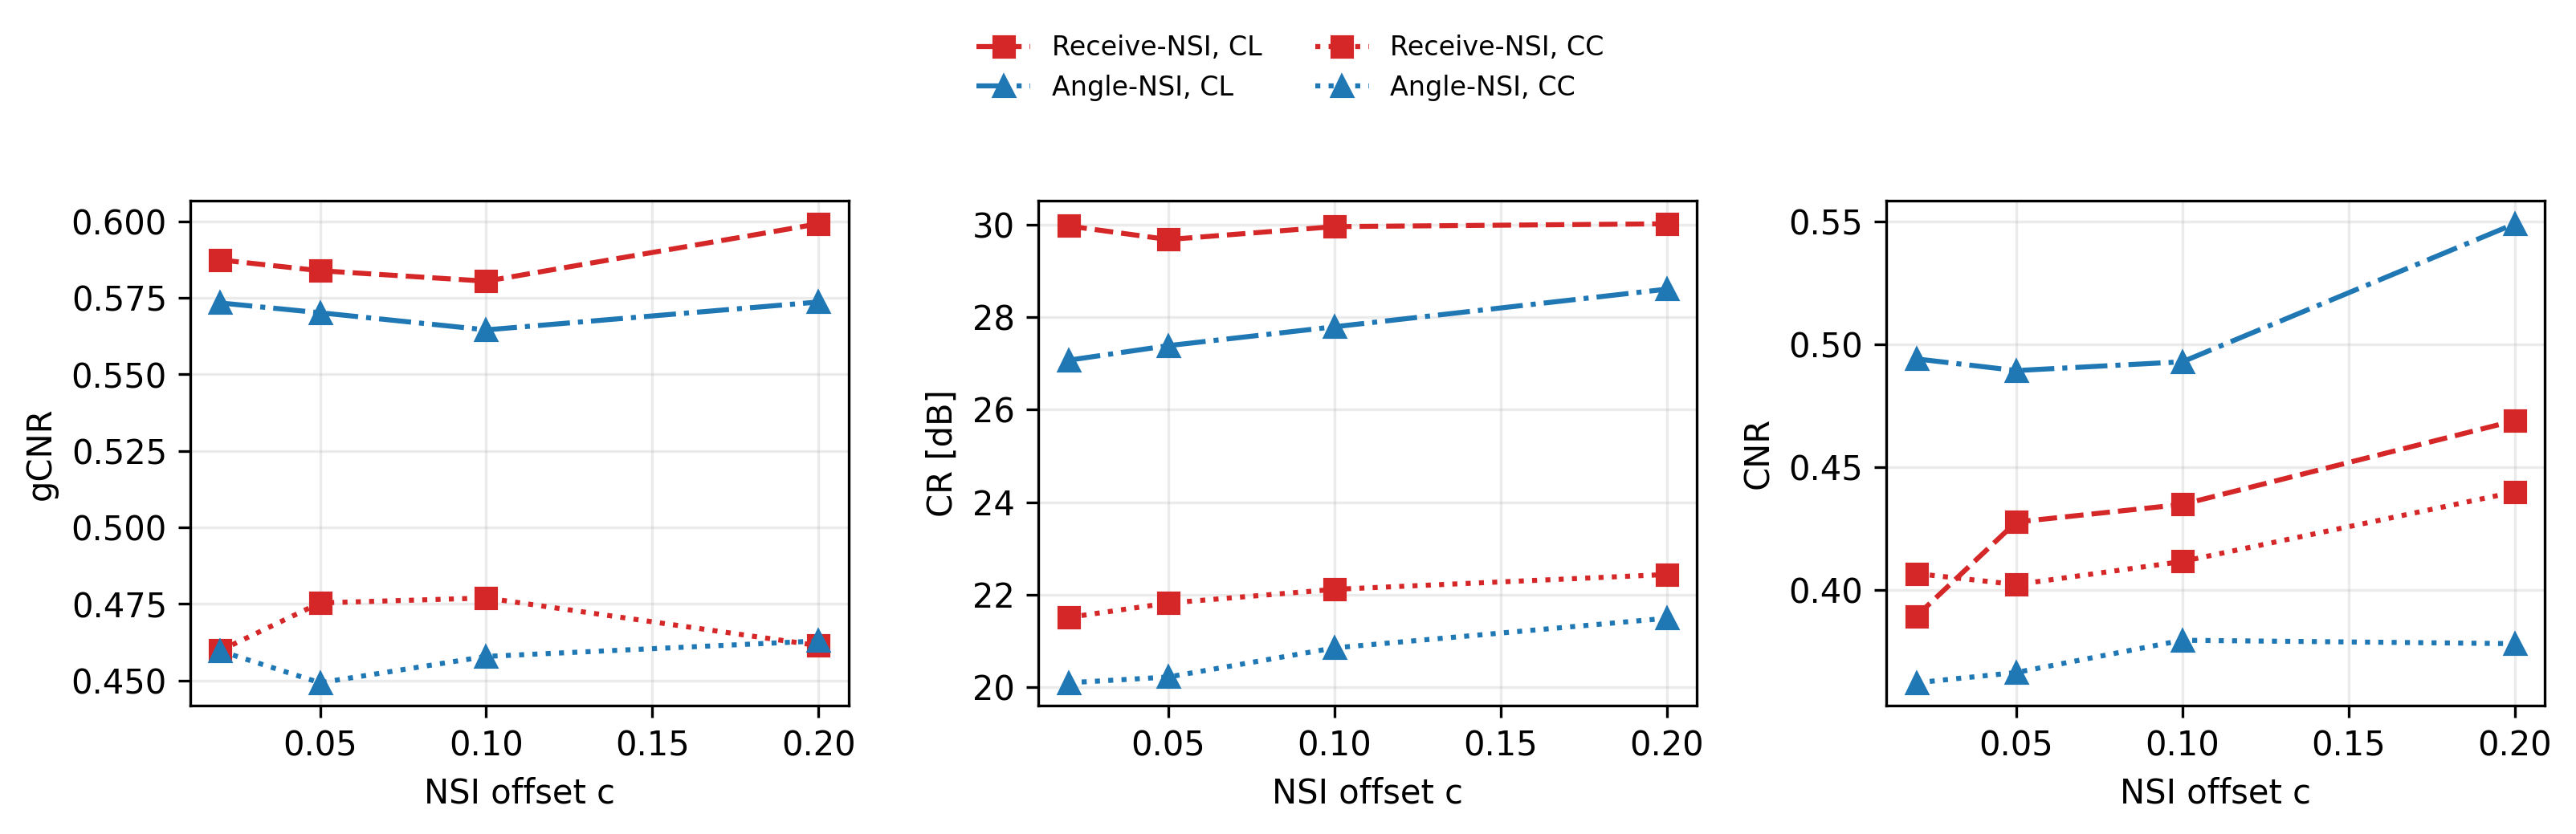
\includegraphics[width=0.92\textwidth]{supplementary/figureS8_carotid_c_sensitivity.png}}{%
\fbox{\parbox{0.85\textwidth}{\centering\revisionpending:\ carotid $c$-sensitivity figure}}}
\caption{Carotid gCNR, contrast ratio and conventional CNR versus $c$ for both
views and both NSI domains.}
\label{fig:s8}
\end{figure}

\clearpage
\section*{S9. Experimental-PSF sensitivity to the NSI offset}

Mean near-axis lateral width and peak-to-local-background level were recomputed
for the five measured PICMUS point targets at every $c$ value.

\begin{figure}[h]
\centering
\IfFileExists{supplementary/figureS9_experimental_psf_c_sensitivity.png}{%
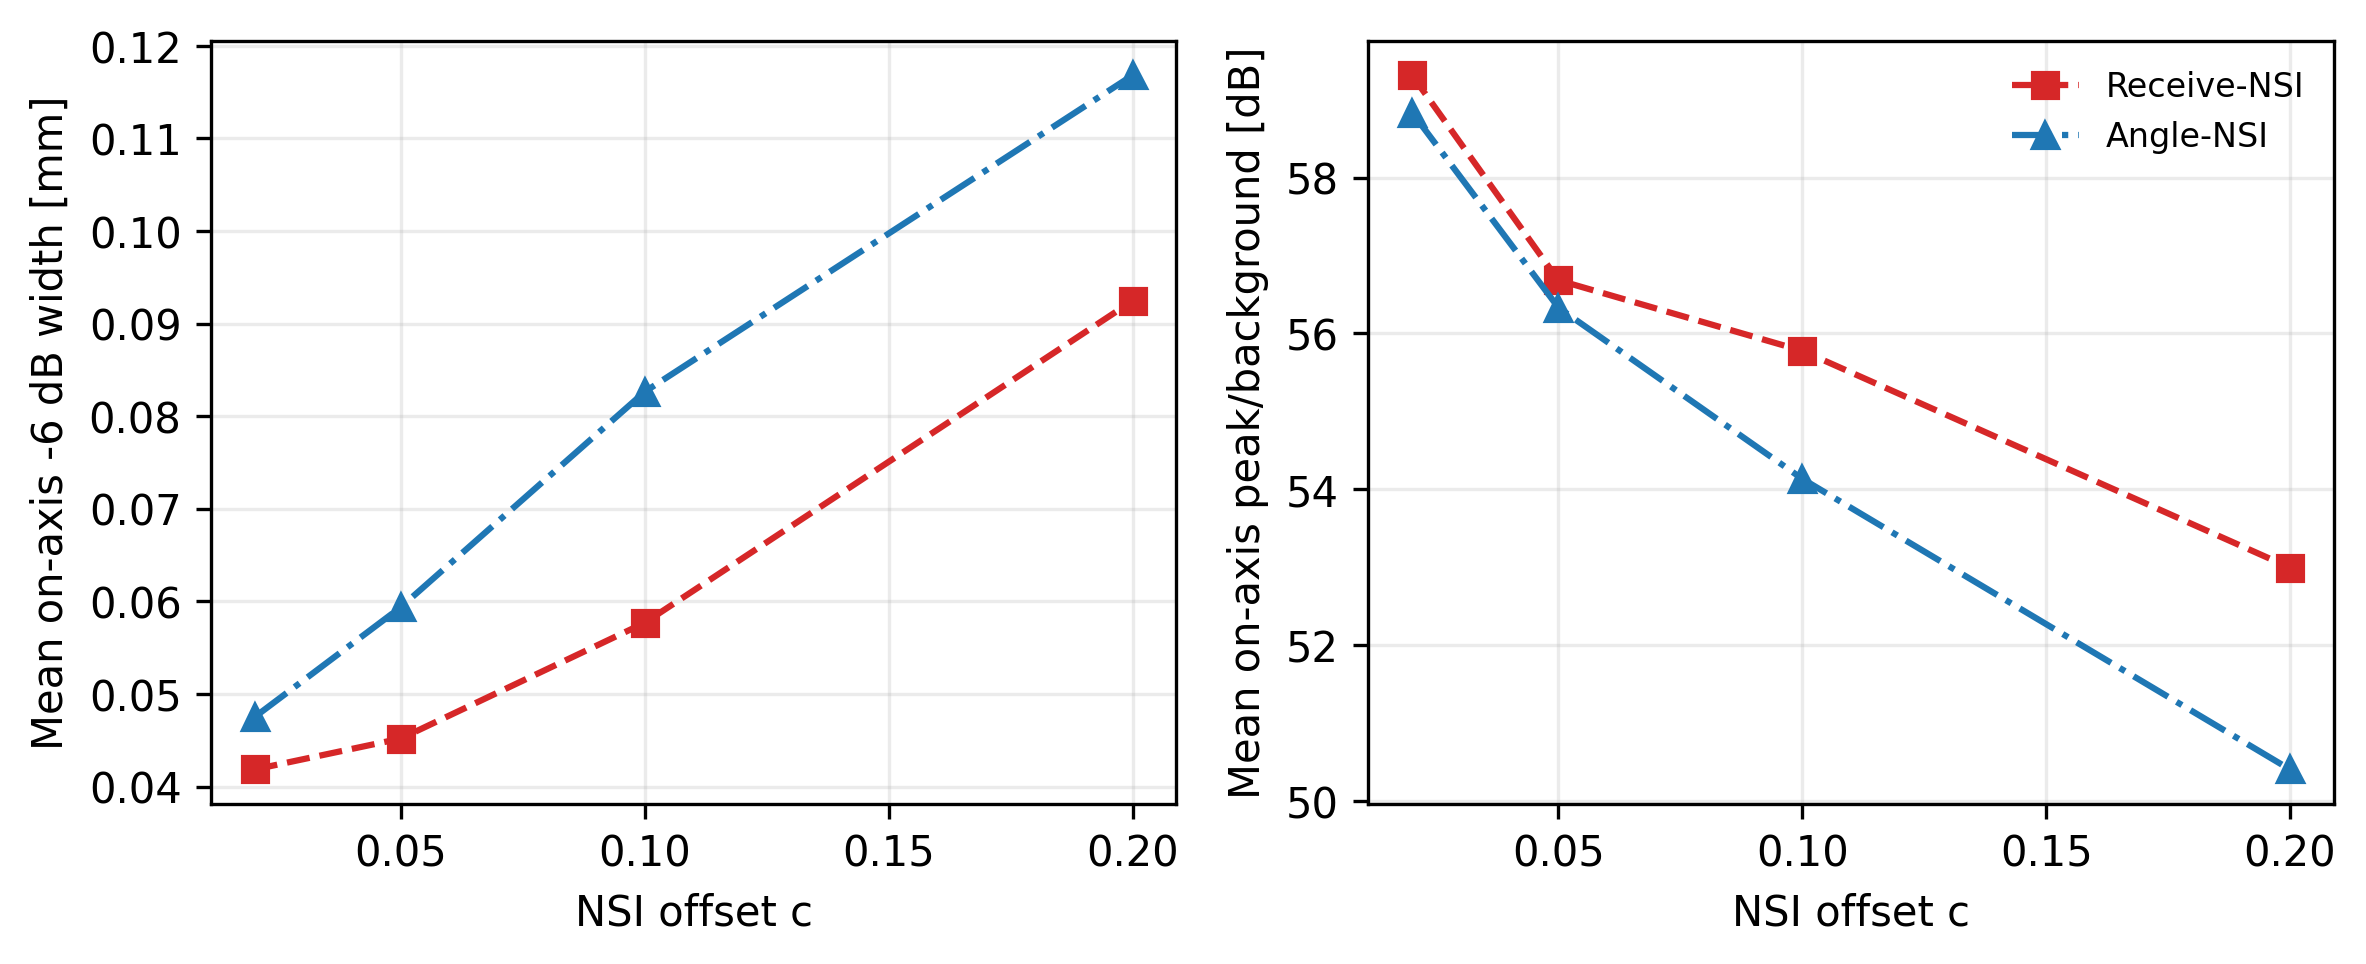
\includegraphics[width=0.90\textwidth]{supplementary/figureS9_experimental_psf_c_sensitivity.png}}{%
\fbox{\parbox{0.85\textwidth}{\centering\revisionpending:\ experimental-PSF $c$-sensitivity figure}}}
\caption{Mean near-axis experimental lateral width and
peak-to-local-background level versus $c$.}
\label{fig:s9}
\end{figure}

\clearpage
\section*{S10. CF-DAS, MV and DMAS definitions and fixed settings}

Let $x_{k,m}(\mathbf r)$ denote the focused receive-element sample for transmit
angle $k$, active element $m$ and image point $\mathbf r$, and let
$M_{\mathrm{active}}$ be the local dynamic-aperture element count. The
coherence-factor-weighted DAS (CF-DAS) output was formed separately for every
transmit angle as
\begin{equation}
\operatorname{CF}_{k}(\mathbf r)=
\frac{|\sum_m x_{k,m}(\mathbf r)|^2}
{M_{\mathrm{active}}\sum_m|x_{k,m}(\mathbf r)|^2},\qquad
y_{k,\mathrm{CF}}=\operatorname{CF}_{k}\sum_m x_{k,m},
\end{equation}
before coherent angular compounding. This is the conventional coherence factor,
equivalent to the DC-only limit of the generalized coherence factor described
by Li and Li. The implementation uses only that DC component.

For minimum variance (MV), every active aperture was divided into all
overlapping contiguous subarrays. Their length was
$L=\lfloor M_{\mathrm{active}}/2\rfloor$. With focused steering vector
$\mathbf 1$, the weights were
\begin{equation}
\mathbf w=\frac{\widehat{\mathbf R}^{-1}\mathbf 1}
{\mathbf 1^{\mathrm H}\widehat{\mathbf R}^{-1}\mathbf 1},\qquad
\widehat{\mathbf R}\leftarrow\widehat{\mathbf R}+
\frac{\operatorname{tr}(\widehat{\mathbf R})}{100L}\mathbf I .
\end{equation}
Subarray outputs were averaged and scaled by $M_{\mathrm{active}}$ before
angular compounding. Forward--backward averaging was omitted. Experimental point targets
used $K=0$; both carotid views used a nine-sample window
($K=4$ on either side) from the fixed 1.5-wavelength rule.

Delay-multiply-and-sum (DMAS) used focused real RF. The signed square-root
samples were
\begin{equation}
u_{k,m}=\operatorname{sign}(x_{k,m})\sqrt{|x_{k,m}|}.
\end{equation}
Their pair sum was
\begin{equation}
q_k=\sum_{i<j}u_{k,i}u_{k,j}
=\frac{(\sum_m u_{k,m})^2-\sum_m u_{k,m}^2}{2}.
\end{equation}
The identity gives the exact pair sum in $O(M)$ operations. Pair sums were
coherently accumulated over angles, filtered along depth with a 60 dB Kaiser
FIR having stop/pass/pass/stop edges $(1.50,1.75,2.50,2.75)f_0$, and converted
to an analytic envelope. The fixed filtering is the standard DMAS
implementation described by Matrone \textit{et al.}; the method is labelled
DMAS throughout the manuscript.

All six methods used the same F-number-1 dynamic receive aperture, receive
delays and linear interpolation. The Python/CuPy implementations followed the
cited formulations and were checked against the corresponding USTB reference
implementations. Every parameter was fixed before the reported outcome.
For the full-phantom overview, the common display spacing was 0.05 mm laterally
and 0.10 mm axially. MV used 0.15 mm lateral sampling and DMAS used 0.10 mm
lateral by 0.02 mm axial sampling before bilinear display resampling. Point-target widths used separate directly beamformed fine profiles.

\begin{table}[h]
\centering
\caption{Fixed implementation choices for the three added receive-domain
comparators. $K$ is the axial covariance half-window in samples.}
\label{tab:s10-parameters}
\begin{tabular}{@{}lp{0.72\linewidth}@{}}
\toprule
Method & Fixed implementation choices \\
\midrule
CF-DAS & Receive-aperture CF per transmit angle; no fitted parameter. \\
MV & $L=\lfloor M_{\mathrm{active}}/2\rfloor$; all overlapping subarrays; loading $\mathrm{tr}(R)/(100L)$; $K=0$ for point targets and $K=4$ (CC), $K=4$ (CL). \\
DMAS & Signed square-root products for $i<j$; fixed Kaiser band-pass around $2f_0$; analytic envelope. \\
\bottomrule
\end{tabular}

\end{table}

\clearpage
\section*{S11. Local experimental responses and complete metrics}

The full seven-target phantom is shown in main figure 2.

Table~\ref{tab:s11-psf}
reports all seven targets for the six methods, with target positions in the
first column.

Quantitative measurements used identical $1.6\times1.6$ mm local maps with
0.02 mm spacing. Lateral profiles were evaluated at the nominal target depth,
and axial profiles at its nominal lateral position. IQ methods used directly
beamformed profiles with 0.002 mm lateral and 0.005 mm axial spacing. DMAS used
0.005 mm lateral and 0.02 mm axial sampling before profile resampling. 

Widths describe the connected $-6$ dB lobe around a target-proximal peak;
localization uses the strongest point in the local two-dimensional map.
Peak/background is $20\log_{10}(P_{\max}/P_{\mathrm{median}})$, where
$P_{\max}$ is the local map peak and $P_{\mathrm{median}}$ is the median
envelope amplitude outside a 0.35 mm radius around the nominal target in the
same map. Main table 2 reports means and sample standard deviations across the
seven target-wise measurements; peak/background values are averaged in dB.

\begin{table}[h]
\centering
\caption{Individual experimental PICMUS response metrics for all seven point
targets and all six methods. The first column gives target number and nominal
position $(x,z)$; $y=0$ for every target. Widths are measured at $-6$ dB on
uncompressed envelopes.}
\label{tab:s11-psf}
\begingroup
\footnotesize
\setlength{\tabcolsep}{4pt}
\resizebox{\textwidth}{!}{\begin{tabular}{@{}llrrrr@{}}
\toprule
Target $(x,z)$ & Method & Lateral width & Axial width & Localisation error & Peak/background \\
(mm) & & (mm) & (mm) & (mm) & (dB) \\
\midrule
1: $(-0.48,9.6)$ & DAS & 0.4328 & 0.5555 & 0.1217 & 26.51 \\
 & CF-DAS & 0.3049 & 0.5240 & 0.0894 & 46.12 \\
 & MV & 0.5074 & 0.8732 & 0.1720 & 17.80 \\
 & DMAS & 0.2461 & 0.5312 & 0.1217 & 37.51 \\
 & Receive-NSI & 0.0233 & 0.5373 & 0.1020 & 59.56 \\
 & Angle-NSI & 0.0369 & 0.5186 & 0.0825 & 58.12 \\
\midrule
2: $(-0.37,18.7)$ & DAS & 0.4561 & 0.5275 & 0.0894 & 26.13 \\
 & CF-DAS & 0.3172 & 0.4599 & 0.0600 & 48.03 \\
 & MV & 0.4689 & 0.5051 & 0.0721 & 21.19 \\
 & DMAS & 0.2532 & 0.4911 & 0.0894 & 36.26 \\
 & Receive-NSI & 0.0499 & 0.5134 & 0.1020 & 54.02 \\
 & Angle-NSI & 0.0707 & 0.5244 & 0.1612 & 56.10 \\
\midrule
3: $(-0.37,28.0)$ & DAS & 0.4873 & 0.5580 & 0.0721 & 26.73 \\
 & CF-DAS & 0.3367 & 0.4276 & 0.0600 & 55.78 \\
 & MV & 0.4012 & 0.7961 & 0.1523 & 24.13 \\
 & DMAS & 0.2805 & 0.5236 & 0.0721 & 35.66 \\
 & Receive-NSI & 0.0377 & 0.5915 & 0.3688 & 60.93 \\
 & Angle-NSI & 0.0570 & 0.5370 & 0.0825 & 58.33 \\
\midrule
4: $(-0.20,37.6)$ & DAS & 0.5732 & 0.5914 & 0.1342 & 26.91 \\
 & CF-DAS & 0.4211 & 0.4658 & 0.0721 & 51.28 \\
 & MV & 0.4132 & 0.5721 & 0.1166 & 25.57 \\
 & DMAS & 0.3496 & 0.6009 & 0.1166 & 29.19 \\
 & Receive-NSI & 0.0636 & 0.6723 & 0.1414 & 53.58 \\
 & Angle-NSI & 0.0707 & 0.5860 & 0.3298 & 53.17 \\
\midrule
5: $(-0.10,47.0)$ & DAS & 0.5388 & 0.5918 & 0.0447 & 26.60 \\
 & CF-DAS & 0.3912 & 0.5509 & 0.0400 & 44.62 \\
 & MV & 0.4490 & 0.5498 & 0.1131 & 28.75 \\
 & DMAS & 0.3360 & 0.6146 & 0.0566 & 32.15 \\
 & Receive-NSI & 0.0515 & 0.6538 & 0.0632 & 55.33 \\
 & Angle-NSI & 0.0616 & 0.6890 & 0.3622 & 55.95 \\
\midrule
6: $(-10.50,37.5)$ & DAS & 0.6247 & 0.5661 & 0.0800 & 29.12 \\
 & CF-DAS & 0.4784 & 0.4781 & 0.0800 & 55.55 \\
 & MV & 0.3824 & 0.7845 & 0.0849 & 26.80 \\
 & DMAS & 0.4067 & 0.5775 & 0.0800 & 32.18 \\
 & Receive-NSI & 0.0584 & 0.6383 & 0.1709 & 60.81 \\
 & Angle-NSI & 0.1339 & 0.3923 & 0.1281 & 47.06 \\
\midrule
7: $(9.80,37.6)$ & DAS & 0.6454 & 0.5928 & 0.0632 & 24.83 \\
 & CF-DAS & 0.4855 & 0.4829 & 0.0825 & 48.79 \\
 & MV & 0.6061 & 0.8728 & 0.0600 & 19.69 \\
 & DMAS & 0.6297 & 0.5932 & 0.0894 & 26.94 \\
 & Receive-NSI & 0.0717 & 0.6000 & 0.2209 & 55.01 \\
 & Angle-NSI & 0.0600 & 0.3690 & 0.0447 & 58.35 \\
\bottomrule
\end{tabular}
}
\endgroup
\end{table}




\clearpage
\section*{S12. Experimental inclusion gCNR}

The bright inclusion on the left of the resolution phantom was compared with
background using two fixed 2 mm radius circles, centered at $(x,z)=(-10.5,27.5)$
and $(10.5,27.5)$ mm. The inclusion region was selected inside the visible
boundary on the DAS image; the background was placed at the same depth and
mirrored lateral position. Identical masks were used for all six methods,
containing 2502 inclusion and 2503 background pixels on the common overview
grid. The native reconstruction grids and display resampling are specified in
section S10. No further image smoothing or reconstruction was applied.

The existing carotid gCNR estimator was used: $\mathrm{gCNR}=1-\sum_j
\min(p_{\mathrm{inclusion},j},p_{\mathrm{background},j})$, where each histogram
was normalized to unit probability. Both regions used the same 100 equally
spaced log-envelope bins spanning their combined range, with the pipeline's
120 dB numerical floor. The 60 dB display cutoff was not used for measurement.
The Table 2 gCNR values describe one region pair per method and are separate
from the seven-target PSF averages.

Varying the radius from 1.5 to 2.25 mm, using 50--200 bins, or shifting the
paired centers by up to 0.25 mm preserved the lower gCNR of both NSI methods
compared with the other four methods. Checks using linear-envelope and pooled
quantile histograms gave the same ordering between these groups. These results
describe this inclusion in one acquisition.

\begin{figure}[h]
\centering
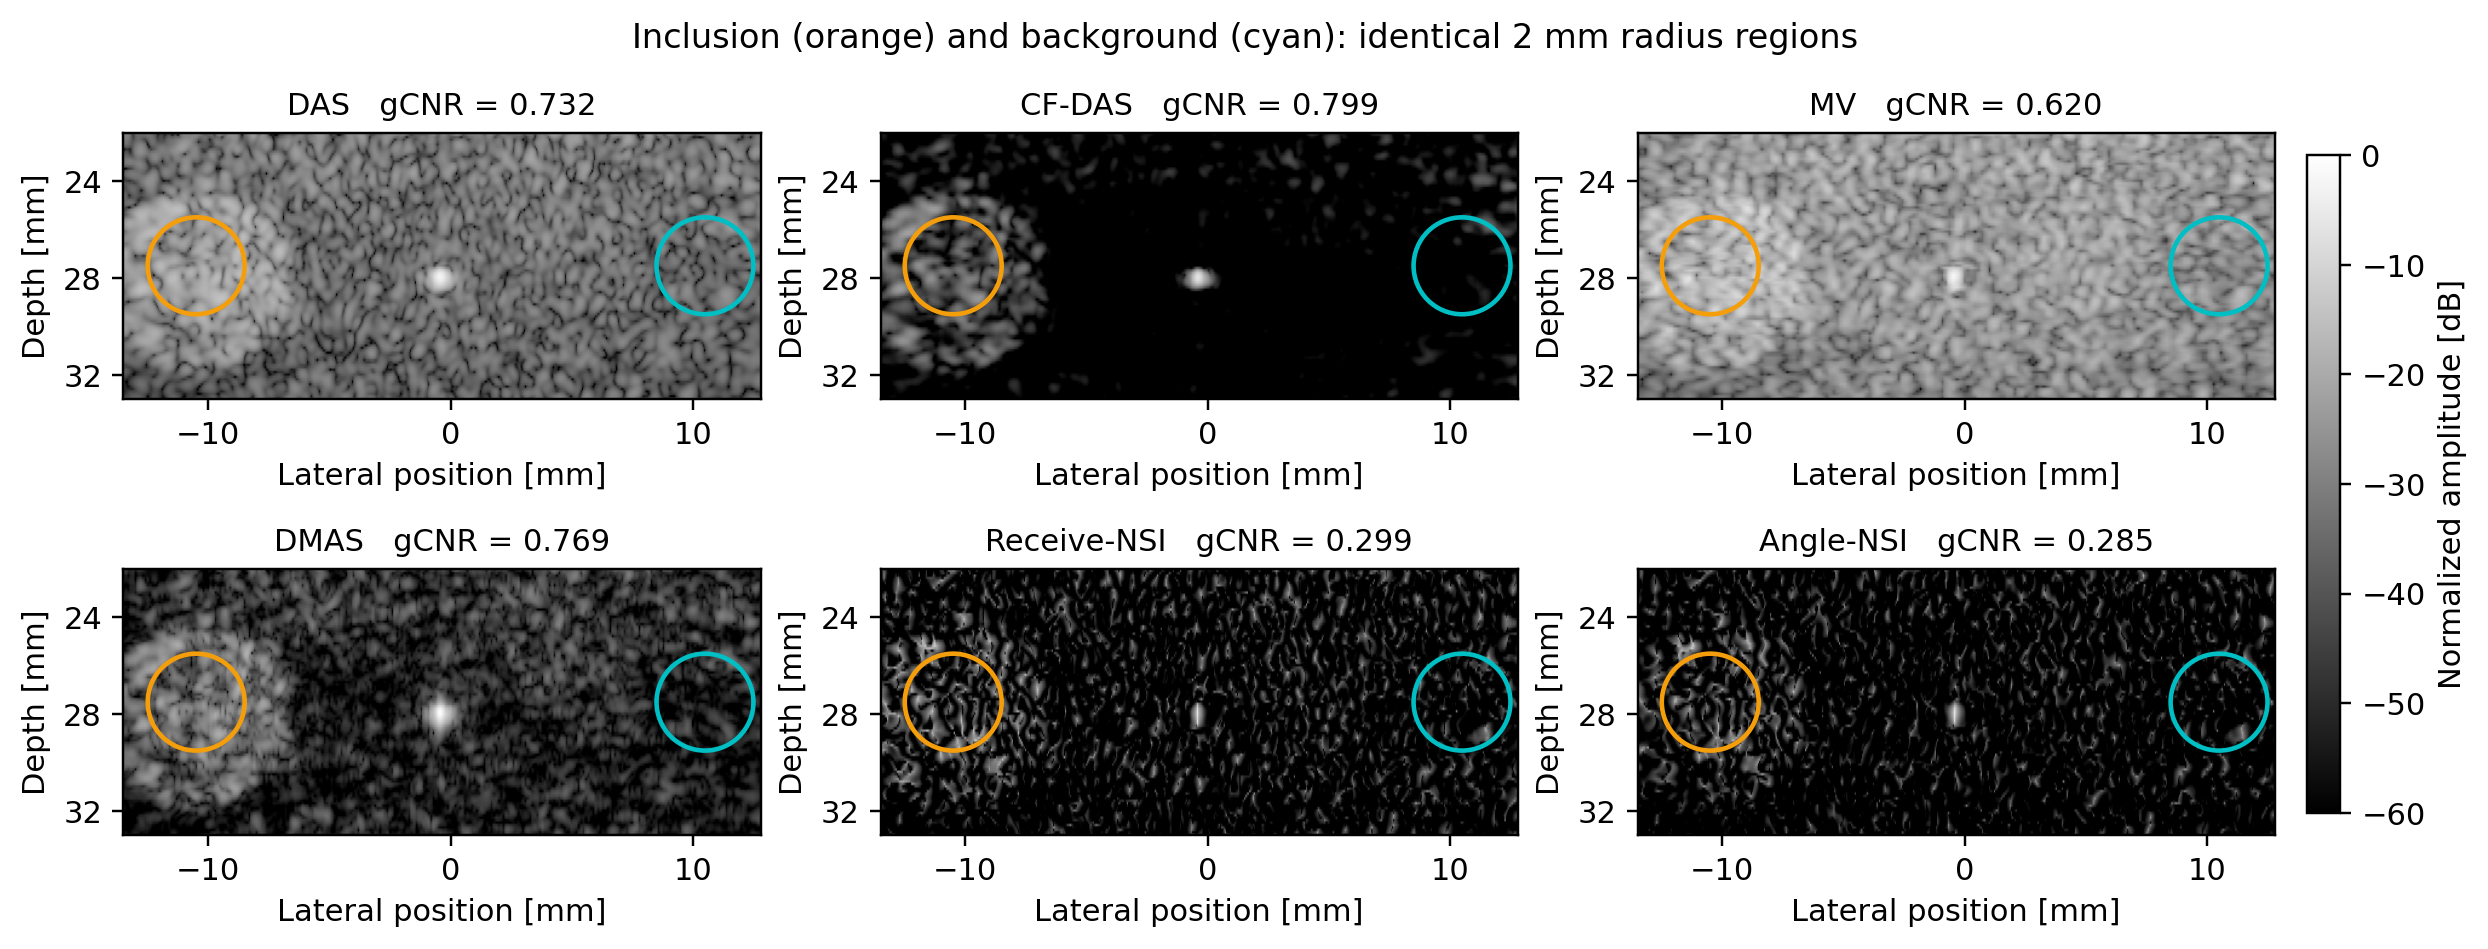
\includegraphics[width=\textwidth]{supplementary/figureS13_picmus_inclusion_rois.png}
\caption{Inclusion (orange) and background (cyan) regions used for the phantom
gCNR column in main table 2. Every circle has a 2 mm radius, and its position is
fixed across methods. The cropped images are normalized independently and
shown over 60 dB; gCNR uses the numerical envelopes as described above.}
\label{fig:inclusion-rois}
\end{figure}

\clearpage
\section*{S13. Carotid contrast metrics}

Because nonlinear beamformers can alter dynamic range, gCNR is the primary
distributional contrast metric. Contrast ratio ($20\log_{10}(\mu_{\rm tissue}/\mu_{\rm lumen})$) and conventional CNR ($|\mu_{\rm tissue}-\mu_{\rm lumen}|/(\sigma_{\rm tissue}^2+
\sigma_{\rm lumen}^2)^{1/2}$) are computed on linear envelopes and included in table~\ref{tab:s11-carotid} for comparison with previous NSI work.
The regions are the fixed lumen and surrounding-tissue regions shown in main
figure 4.

\begin{table}[h]
\centering
\caption{Carotid metrics for the six methods in the main-figure regions.}
\label{tab:s11-carotid}
\resizebox{\textwidth}{!}{\begin{tabular}{@{}lrrrrrr@{}}
\toprule
& \multicolumn{3}{c}{Cross-sectional} & \multicolumn{3}{c}{Longitudinal} \\
\cmidrule(lr){2-4}\cmidrule(l){5-7}
Method & gCNR & CR (dB) & CNR & gCNR & CR (dB) & CNR \\
\midrule
DAS & 0.7342 & 18.98 & 0.8310 & 0.9502 & 28.24 & 1.1965 \\
CF-DAS & 0.9383 & 36.10 & 0.6776 & 0.8177 & 27.90 & 0.7248 \\
MV & 0.7335 & 17.33 & 0.8917 & 0.9637 & 27.13 & 1.2325 \\
DMAS & 0.7539 & 18.28 & 0.7403 & 0.9623 & 32.30 & 0.9417 \\
Receive-NSI & 0.4579 & 21.25 & 0.3931 & 0.5957 & 27.99 & 0.4366 \\
Angle-NSI & 0.4481 & 22.86 & 0.2315 & 0.5942 & 28.25 & 0.3847 \\
\bottomrule
\end{tabular}
}
\end{table}

\clearpage
\section*{S14. Timing controls and six-method kernel benchmark}

The primary end-to-end benchmark transfers one raw complex64 IQ array for
every method and forms Receive-NSI weights on the device. The preloaded control
times kernels with all inputs resident on the GPU. The host-stacked control
transfers two channel-sized Receive-NSI fields and reproduces the interface
boundary used for the original 18.0\% comparison. These controls isolate
transfer and interface choices and are not the primary end-to-end result.

\begin{table}[h]
\centering
\caption{Preloaded-kernel and host-stacked-input controls. Transfer is the
exact logical timed payload; the within-control ratio is relative to DAS.}
\label{tab:s12-controls}
\resizebox{\textwidth}{!}{\begin{tabular}{@{}llrrr@{}}
\toprule
Control & Method & Median (ms) & Relative to DAS & Transfer (MiB) \\
\midrule
Preloaded kernel & DAS & 6.66 & 1.000 & 0.00 \\
Preloaded kernel & Receive-NSI & 10.96 & 1.645 & 0.00 \\
Preloaded kernel & Angle-NSI & 7.60 & 1.141 & 0.00 \\
Host-stacked input & DAS & 22.58 & 1.000 & 36.63 \\
Host-stacked input & Receive-NSI & 31.93 & 1.414 & 70.63 \\
Host-stacked input & Angle-NSI & 23.67 & 1.048 & 36.63 \\
\bottomrule
\end{tabular}
}
\end{table}

The synchronized six-method experiment used 17 angles, 64 receive elements and
an $8\times64$-pixel grid, with delayed complex IQ and real RF tensors already
resident on the NVIDIA RTX A2000. Ten warm-ups preceded 50 repetitions. The
boundary includes each method-specific reduction, the MV covariance and solve,
and the DMAS filtering and Hilbert-transform stages. It excludes raw-data
transfer, delay calculation, interpolation and final device-to-host transfer.

\begin{table}[h]
\centering
\caption{Median post-delay GPU kernel times and leading arithmetic orders.
$M$ is the active element count, $L$ the MV subarray length and $K$ its axial
half-window.}
\label{tab:s12-timing}
\resizebox{\textwidth}{!}{\begin{tabular}{@{}lrrl@{}}
\toprule
Method & Median (ms) & Relative to DAS & Leading order per pixel/angle \\
\midrule
DAS & 0.073 & 1.00 & $O(M)$ \\
CF-DAS & 6.395 & 87.96 & $O(M)$ \\
MV & 416.692 & 5731.34 & $O((2K+1)(M-L+1)L^2+L^3)$ \\
DMAS & 4.175 & 57.42 & $O(M^2)$ direct; $O(M)$ exact identity \\
Receive-NSI & 0.737 & 10.13 & $O(M)$ \\
Angle-NSI & 0.372 & 5.12 & $O(M)$ \\
\bottomrule
\end{tabular}
}
\end{table}

Complete raw runs, medians, bootstrap confidence intervals, configuration
metadata, numerical-equivalence checks and exact byte accounting are supplied
as CSV/JSON files by the public analysis workflow.




\end{document}
